%!TEX root = ../../memoria.tex
\chapter{Solución implementada}

Como se explicó en la \refSection{cap:arquitectura:section:generic_architecture_structure}, fue necesario desarrollar una arquitectura genérica para el desarrollo de aplicaciones en \meteorNAME con el fin de generar código de calidad. Acto seguido se comenzó con la implementación de las siguientes características:

% diseño arquitectura generica
%!TEX root = ../../../memoria.tex
\section{Arquitectura del \frameworkPC}\label{cap:arquitectura:section:arquitectura_framework}

\subsection{\packagesAS}

A continuación se describen las funcionalidades de cada uno de los \packagesAS que actualmente existen. La estructura se encuentra en \refFigura{cap:avances:current_architecture}.

\tikzset{
  basic/.style  = {draw, text width=2cm, drop shadow, font=\sffamily, rectangle},
  root/.style   = {basic, rounded corners=2pt, thin, align=center,
                   fill=green!30},
  level 2/.style = {basic, rounded corners=6pt, thin,align=center, fill=green!60,
                   text width=8em},
  level 3/.style = {basic, thin, align=left, fill=pink!60, text width=6.5em}
}
\begin{figure}[H]
	\centering
	
	
	\begin{tikzpicture}[
	  level 1/.style={sibling distance=40mm},
	  edge from parent/.style={->,draw},
	  >=latex]

	% root of the the initial tree, level 1
	\node[root] {\eframeworkAF}
	% The first level, as children of the initial tree
		child {node[level 2] (c1) {\eframeworkCorePCKG}}
		%child {node[level 2] (c2) {\eframeworkHelloWorldPCKG}}
		child {node[level 2] (c3) {\eframeworkAccountsPCKG}}
		%child {node[level 2] (c4) {rtcom-shipping}}
		child {node[level 2] (c5) {\eframeworkPaypalPCKG}};
		%child {node[level 2] (c6) {\eframeworkGoogleanalPCKG}};
	\end{tikzpicture}
	\caption{\architectureCPT actual de la solución.}
	\label{cap:avances:current_architecture}
\end{figure}
	\begin{itemize}
		\item
			\textbf{\eframeworkAF} es un \frameworkPC \ecommerceCOM desarrollado con \meteorNAME, \nodejsNAME, \mongodbNAME, con un enfoque \reactive y \realTimeINT.
		\item
			\textbf{\eframeworkCorePCKG} corresponde al \coreAS de la solución. Contiene todas aquellas \featuresCPT básicas y \templatesAS a una plataforma \ecommerceCOM tales como manejo de \itemsCOM, \sessionsINT, shipping, ordenes de compra, carro de compra.
		\item
			\textbf{\eframeworkAccountsPCKG} es el \moduleAS para el manejo de cuentas.
		\item
			\textbf{\eframeworkCoreThemePCKG}
		\item
			\textbf{\eframeworkBootstrapThemePCKG}
		\item
			\textbf{\eframeworkShippingPCKG}
		\item
			\textbf{\eframeworkPaypalPCKG}
		
		% \item
		% 	\textbf{\eframeworkHelloWorldPCKG} es un \moduleAS para prueba de conceptos.
	\end{itemize}


La arquitectura descrita en la \refSection{cap:arquitectura:section:generic_arquitectura} fue diseñada para facilitar las implementaciones de cada uno de los \packagesAS que se desarrollen en los proyectos de \meteorNAME. En particular para el proyecto que se desarrolla en este informe se utiliza dicha estructura principalmente en el \packagesAS \coreAS de la aplicación.

\subsubsection{\eframeworkCorePCKG}

Como su nombre lo indica, este \packagesAS corresponde al \coreAS del \frameworkPC conteniendo todas aquellas caracteristicas intrínsecas que dan vida a un sitio \ecommerceCOM. 

\subsubsection{\eframeworkCoreThemePCKG}\label{chapter:section:subsection:package_core_theme}

Este \packagesAS es la base del \bootstrap \themeCPT del \frameworkPC de \ecommerceCOM. Este contiene todos los archivos \lessNAME utilizados para el proceso que genera los archivos \lessNAME personalizado para el \frameworkPC. Este \packagesAS puede ser copiado para crear \themeCPT adicinales para el \frameworkPC \ecommerceCOM.

La implementación de este \packagesAS esta soportada sobre \bootstrapPackage permitiendo sencillamente hacer todas aquellas configuraciones que se desean. \bootstrapPackage permite, entre otras cosas, indicar exactamente cuales son las componentes de \bootstrapNAME que se desean utilizar, así como personalizar e importar el \themeCPT.

A modo de ejemplo, se mostrarán a continuación ejemplos de importaciones de \themesCPT en el \frameworkPC. Para esto se utilizará los \themesCPT gratuitos que proporciona \bootswatchNAME. Esta tarea es muy sencilla, y basta con agregar el \refsource{source:less:generic_bootswatch_theme} al final del arhivo generado por \bootstrapPackage llamado \textbf{custom.reaction.import.less}.

% import codigo 
%%!TEX root = ../../../memoria.tex

\medskip
\begin{lstlisting}[caption= Código genérico para importar \themesCPT de ., label=source:less:generic_bootswatch_theme]
	@import "http://bootswatch.com/THEME_NAME/bootswatch.less";
	@import "http://bootswatch.com/THEME_NAME/variables.less";
\end{lstlisting}
\medskip
\begin{lstlisting}[caption= Código genérico para importar \themesCPT desde \bootswatchNAME, label=source:less:generic_bootswatch_theme]
	@import "http://bootswatch.com/THEME-NAME/bootswatch.less";
	@import "http://bootswatch.com/THEME-NAME/variables.less";
\end{lstlisting}

En donde \textbf{THEME-NAME} corresponde a algún \themeCPT de los disponibles en el sitio de \bootswatchNAME. En particular, los \themesCPT \textbf{\themeSandstone}, \textbf{\themeJournal}, \textbf{\themeCyborg} y \textbf{\themeSuperHero} se pueden apreciar en la \refFigura{figure:bootstrap:theme_standstone}, \ref{figure:bootstrap:theme_journal}, \ref{figure:bootstrap:theme_cyborg} y \ref{figure:bootstrap:theme_superhero} respectivamente.


\begin{figure}[H]
	\centering
	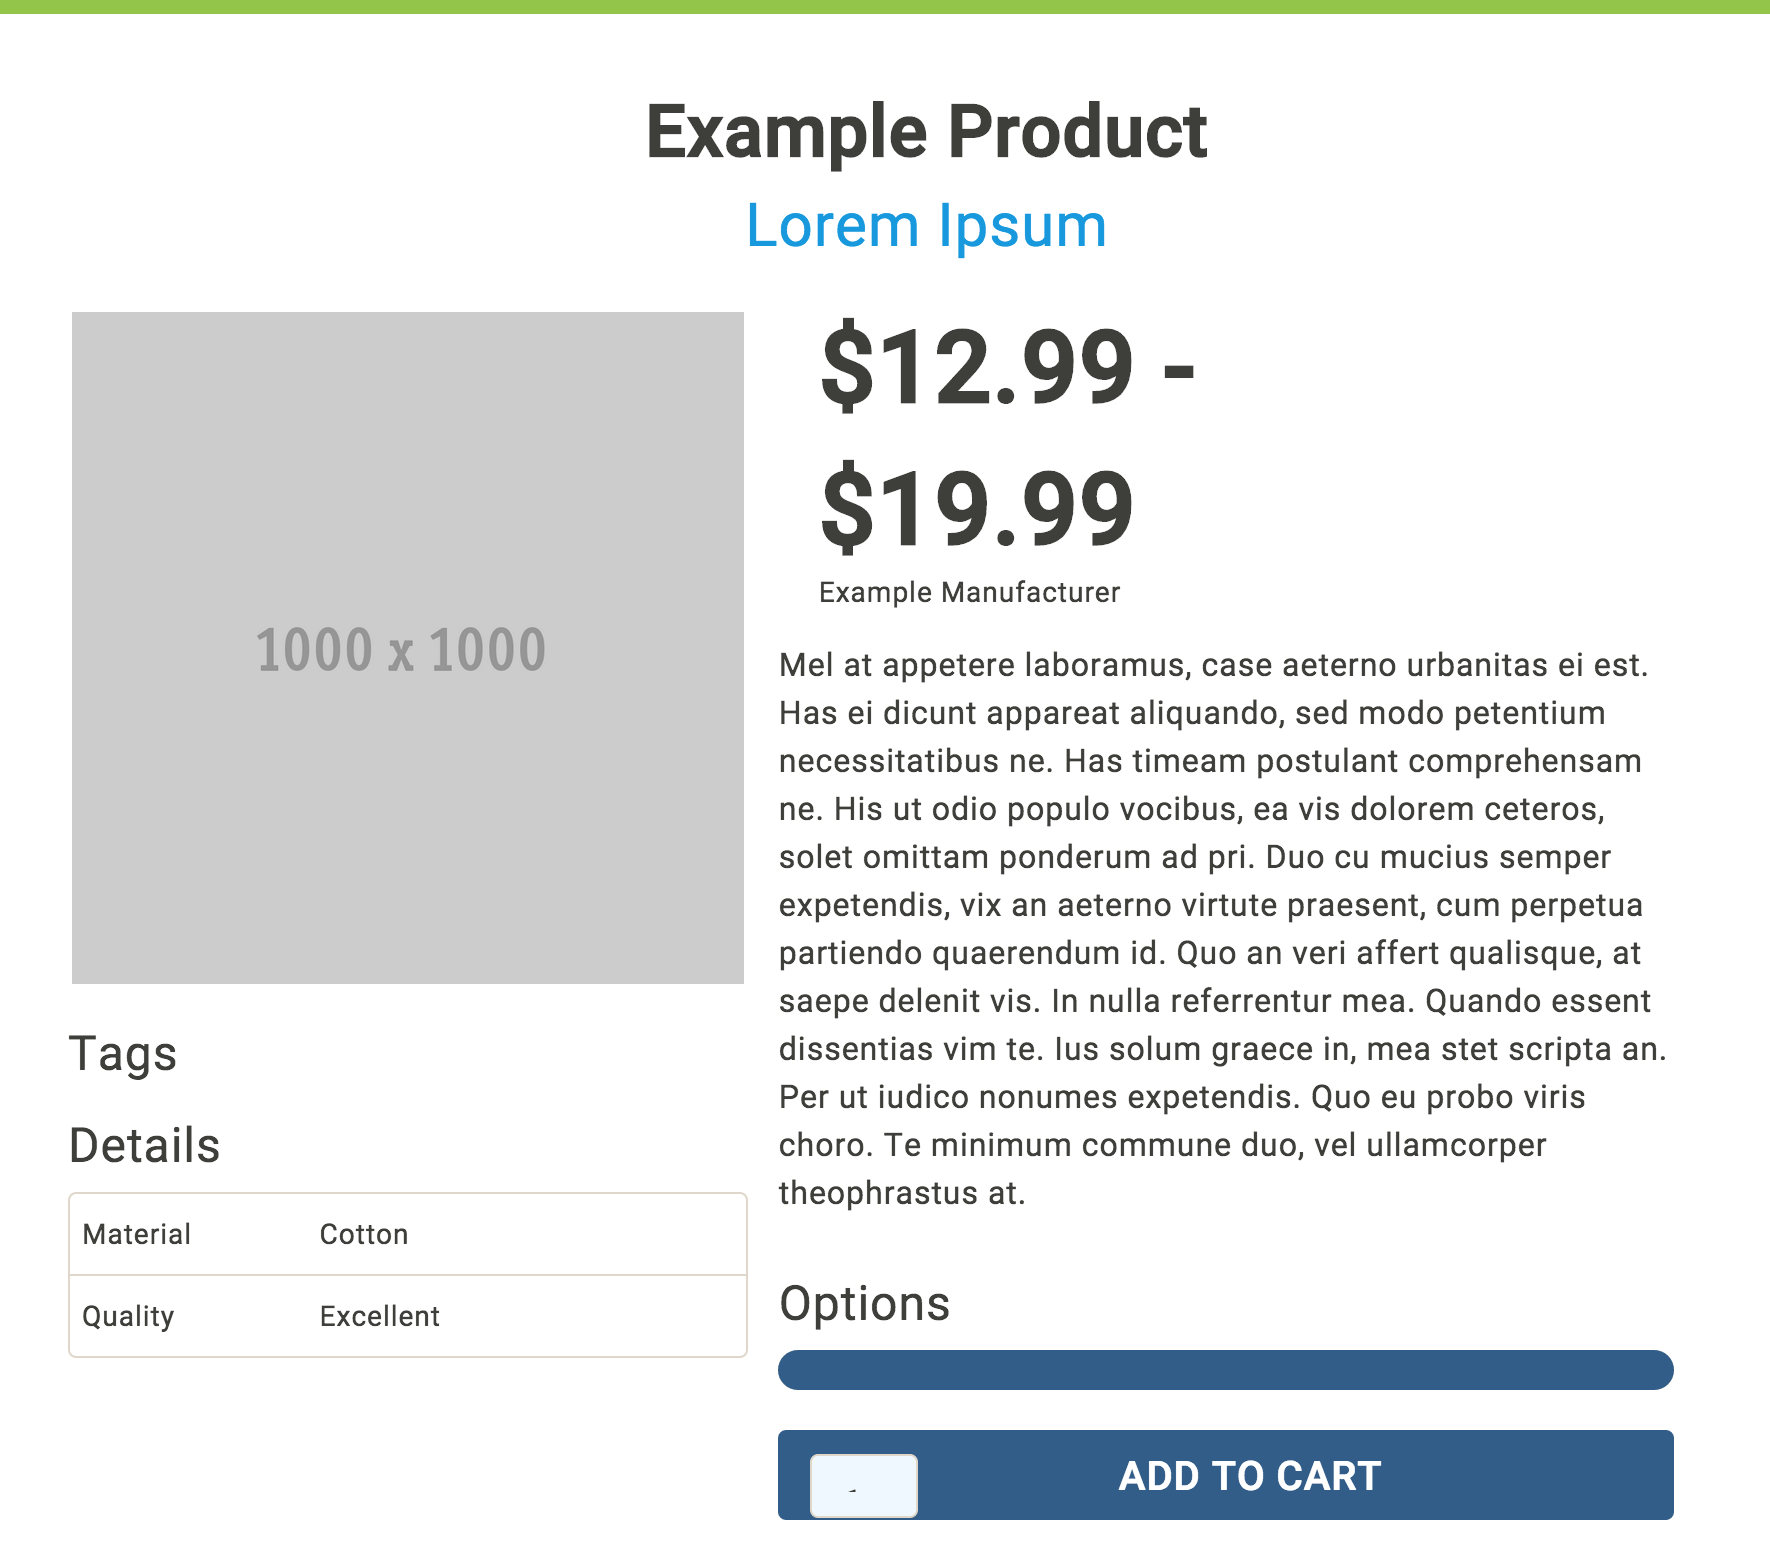
\includegraphics[width=0.6\textwidth]{figuras/bootstrap/bootstrap_theme_sandstone.png}

	\caption{Descripción de un producto utilizando el \themeCPT \textbf{\themeSandstone} del sitio \bootswatchNAME.}
	\label{figure:bootstrap:theme_standstone}
\end{figure}

\begin{figure}[H]
	\centering
	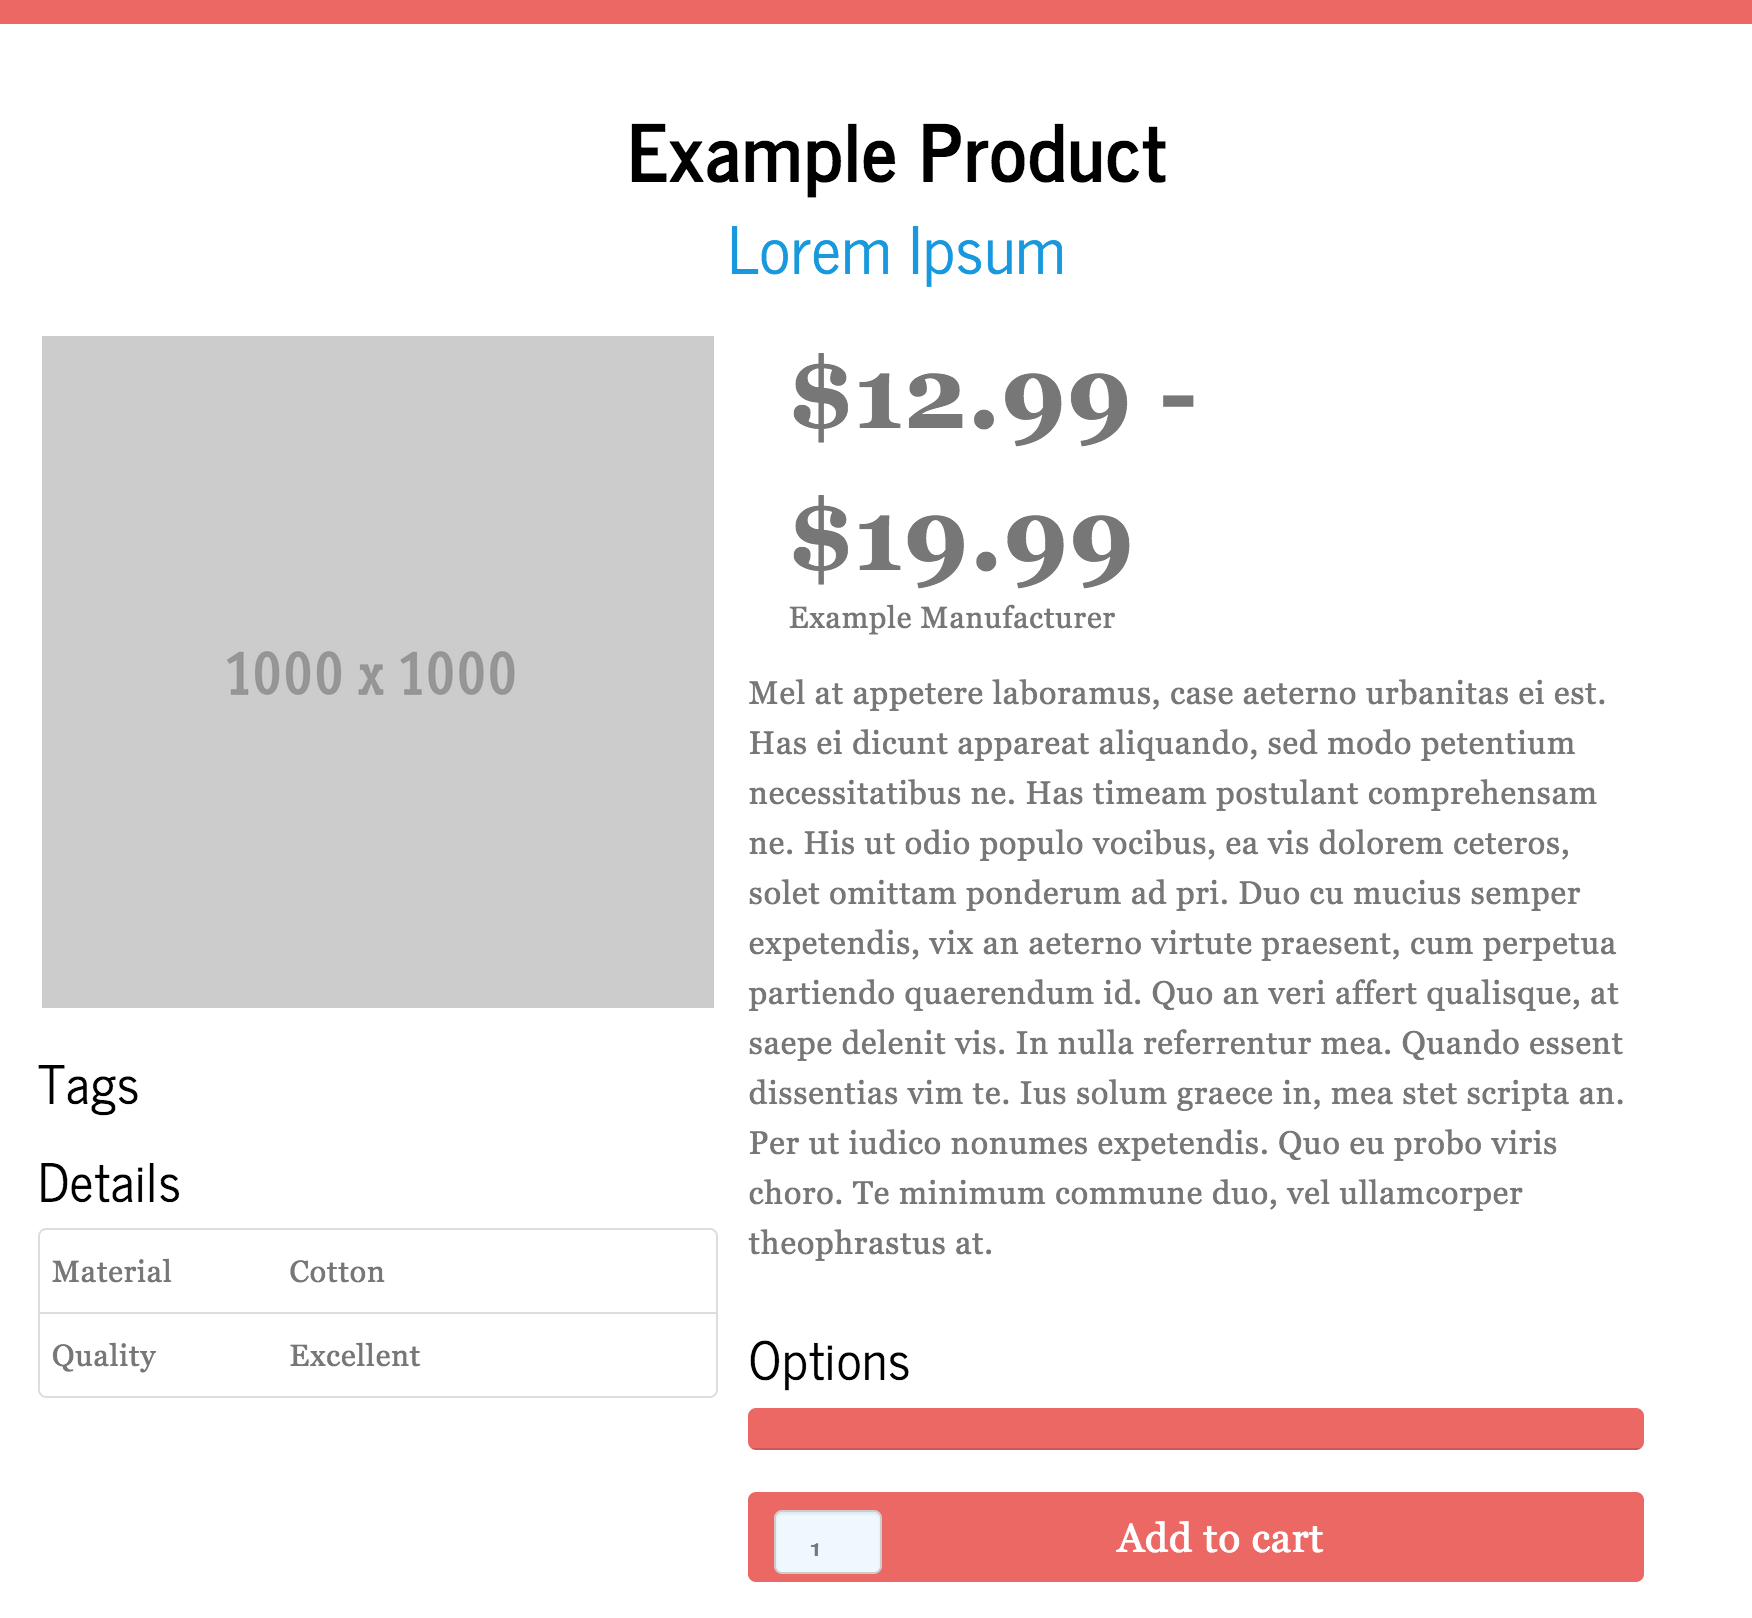
\includegraphics[width=0.6\textwidth]{figuras/bootstrap/bootstrap_theme_journal.png}

	\caption{Descripción de un producto utilizando el \themeCPT \textbf{\themeJournal} del sitio \bootswatchNAME.}
	\label{figure:bootstrap:theme_journal}
\end{figure}

\begin{figure}[H]
	\centering
	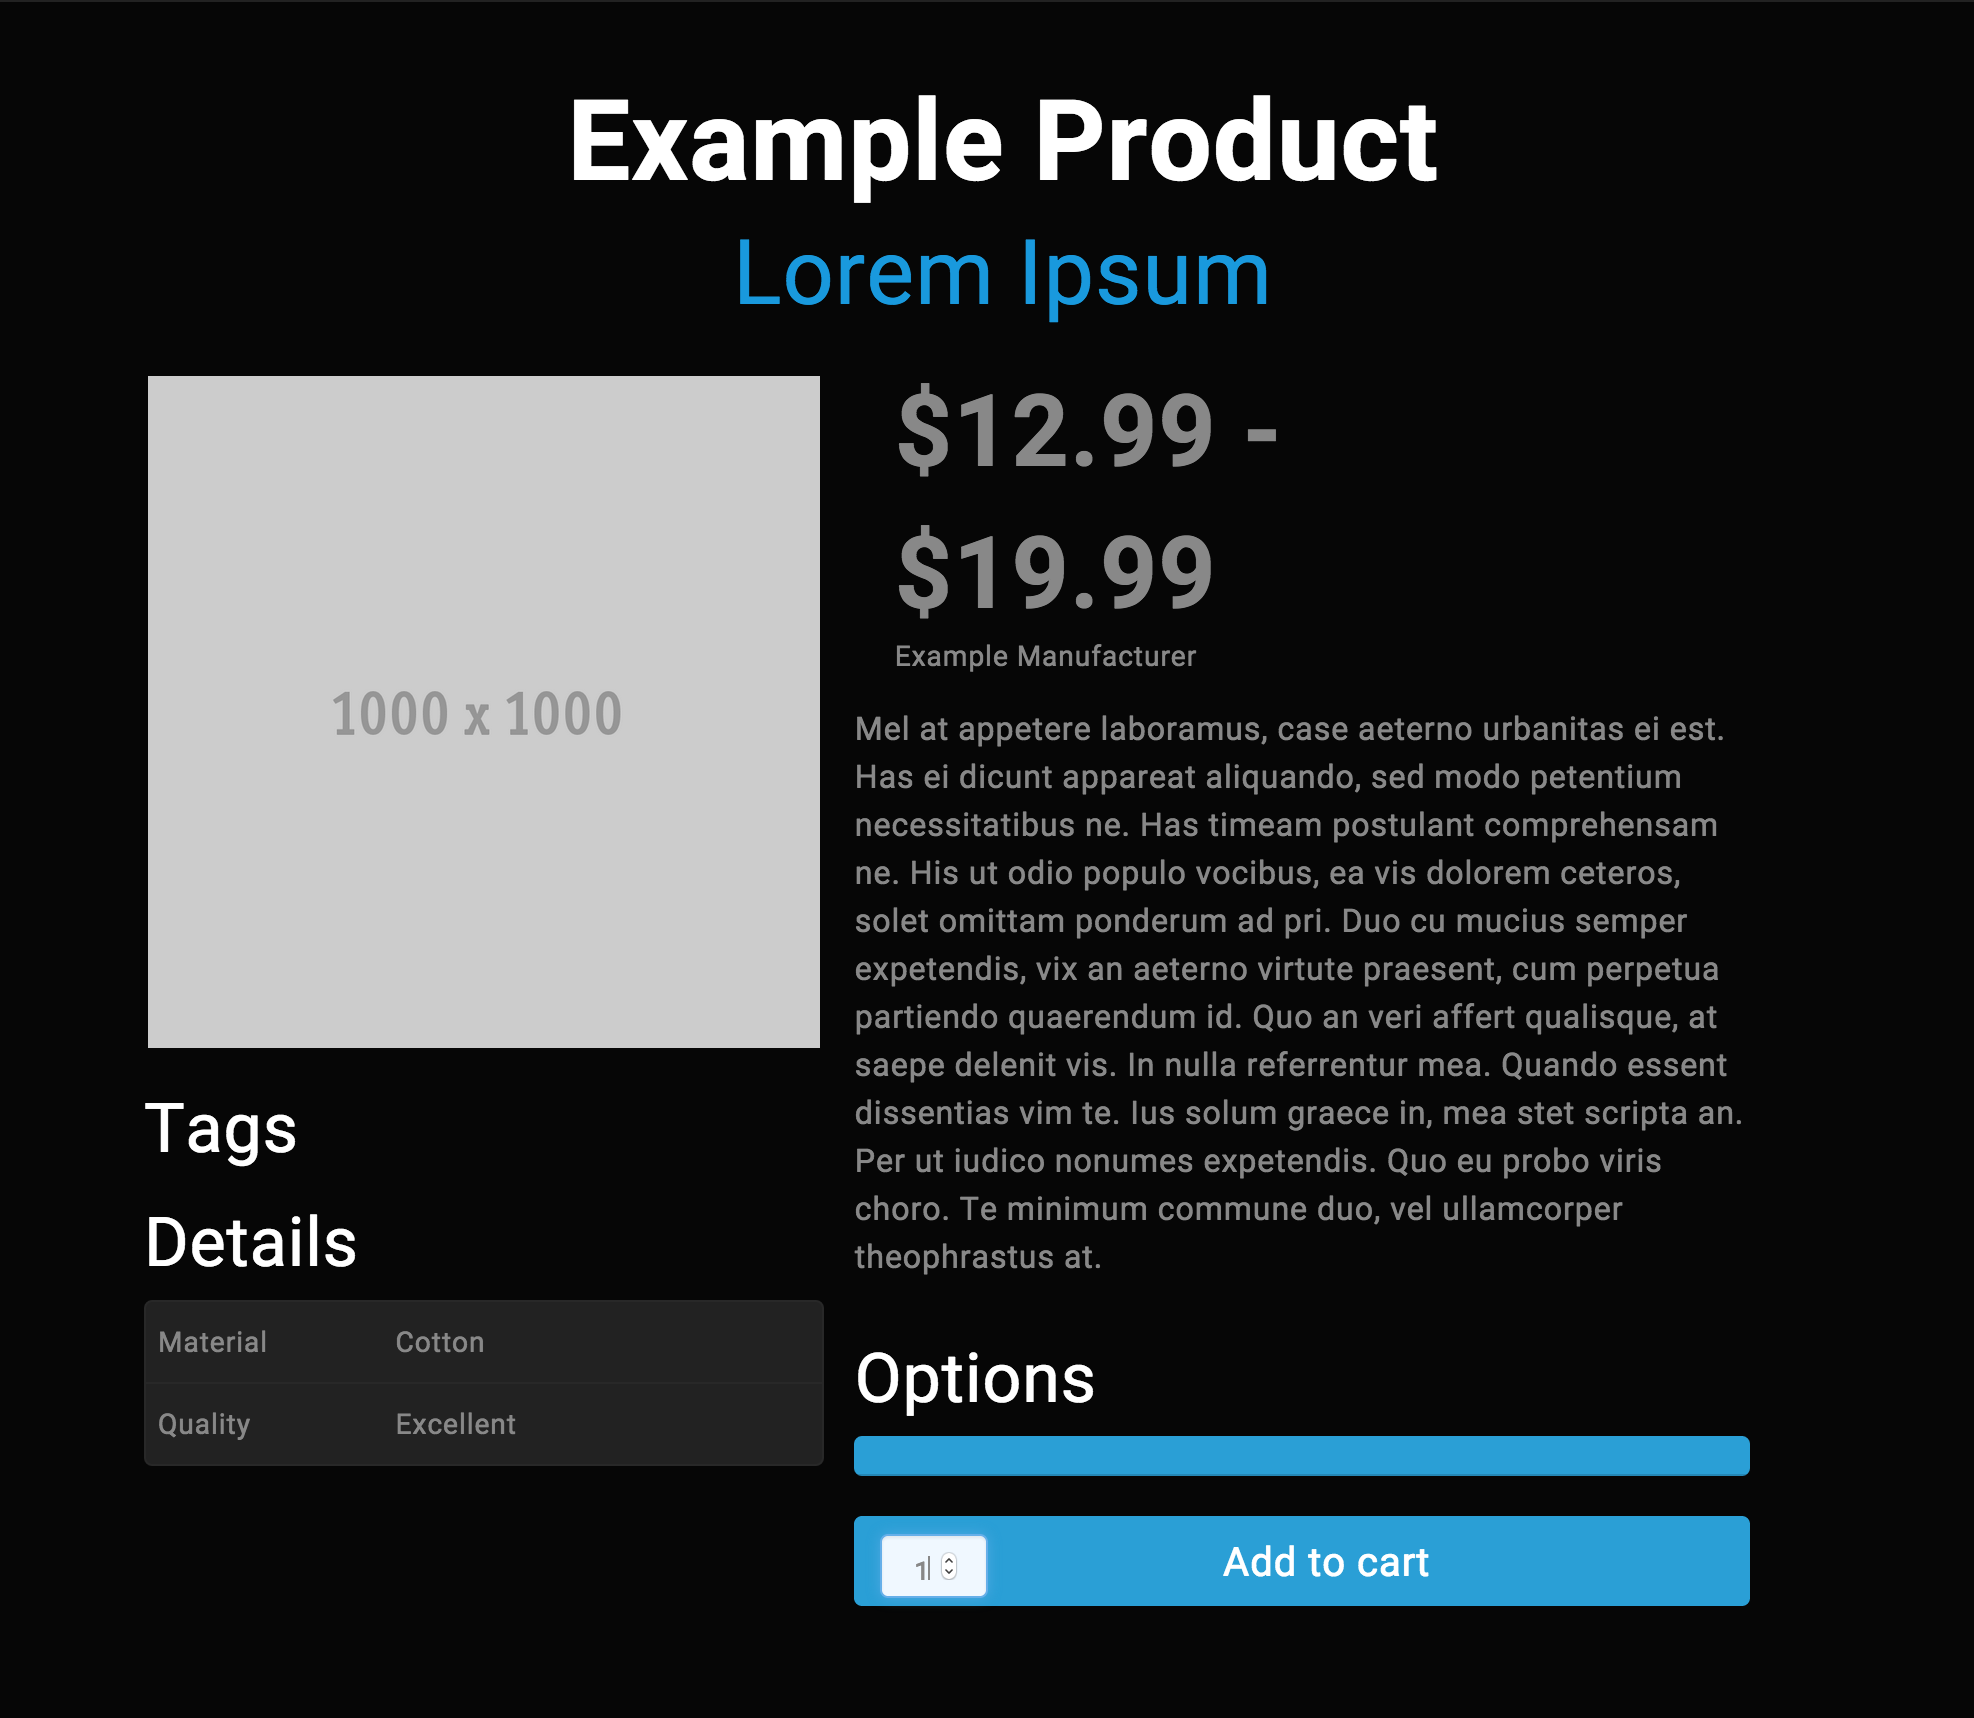
\includegraphics[width=0.6\textwidth]{figuras/bootstrap/bootstrap_theme_cyborg.png}

	\caption{Descripción de un producto utilizando el \themeCPT \textbf{\themeCyborg} del sitio \bootswatchNAME.}
	\label{figure:bootstrap:theme_cyborg}
\end{figure}


\begin{figure}[H]
	\centering
	\includegraphics[width=0.6\textwidth]{figuras/bootstrap/bootstrap_theme_superhero.png}

	\caption{Descripción de un producto utilizando el \themeCPT \textbf{\themeSuperHero} del sitio \bootswatchNAME.}
	\label{figure:bootstrap:theme_superhero}
\end{figure}

\subsubsection{\eframeworkCorePCKG}

% Sección que habla sobre los workflows en el framwork
%!TEX root = ../../../memoria.tex

\subsection{\workflowsCPT}

%TODO
% Introduccion de workflows

Existen una serie de pasos que se pueden experimentar al visitar un sitio \ecommerceCOM, entre los cuales podemos destacar:

	\begin{itemize}
		\item
			\textbf{Shopping Experience}.
		\item
			\textbf{Order Capture} 
		\item
			\textbf{Order Fullfillment} 
		\item
			\textbf{Order processing}
		\item
			\textbf{Shipping} 
		\item
			\textbf{Customer Files} 
		\item
			\textbf{Paymanat Sistems} 
		\item
			\textbf{Customer Service} 
		\item
			\textbf{Accounting} 
		\item
			\textbf{Returning} 
	\end{itemize}


Cada uno de los pasos dentro de un \workflowsCPT puede ser considerado como un estado el cual cambiará dependiendo de los eventos que esten involucrados. Por lo tanto cada uno de estos \workflowsCPT puede ser modelado utilizando una máquina de estados finitos.
Para el caso particular del \frameworkPC para \ecommerceCOM, 4 han sido los \workflowsCPT que han sido implementados utilizando la librería \javaScriptNAME \finiteStateMachine.

\begin{figure}[H]
	\centering
	\includegraphics[width=1.1\textwidth]{figuras/cart_state_machine.jpg}

	\caption{Máquina de estado de carro de compras.}
	\label{figure:cart_state_machine}
\end{figure}


\begin{figure}[H]
	\centering
	\includegraphics[width=0.8\textwidth]{figuras/order_state_machine.jpg}

	\caption{Máquina de estado del estado de una orden.}
	\label{figure:order_state_machine}
\end{figure}



% caracteristicas de una cuenta
%!TEX root = ../../../memoria.tex
\section{Control de Acceso}

Control de acceso limita las acciones directas de un usuario, así como qué programas pueden ejecutarse \cite{sandhu1994access}.
 
%Meteor Accounts
%Meteor Accounts is a complete user account system that you can drop into your application. With one line of code, you can have login, logout, account creation, email validation, password recovery, and login with OAuth providers like Facebook or Twitter.
Existe un sistema completo de cuentas de usuarios, el cual permite hacer \loginCPT(\refFigura{figure:account:signin:form}), \logoutCPT(\refFigura{figure:accounts:logout:form}), creación de cuentas (\refFigura{figure:account:create_account:form}), y recuperación de contraseña (\refFigura{figure:account:reset:form}). 
%Aunque en estricto rigor la recuperación de contraseña momentáneamente corresponde a una contraseña aleatoria generada por la aplicación y enviada al correo.

\subsection{Creación de cuenta de un usuario}\label{chapter:solucionimplementada:accounts:subsection:create}

La creación de una cuenta se ha pensado realizando la menor cantidad de acciones posibles. Agregar acciones innecesarias puede significar que los usuarios desistan y dejen el sitio\cite{online_goodgui_org}. Una de las acciones innecesarias más común es llenar dos campos de un formulario con la misma información: ejemplos de esto son escribir dos veces el \email y la contraseña (ver \refFigura{figure:account:create_account:form_compare}). Históricamente esto ha sido diseñado para prevenir errores de tipeo. Esta ultima situación no es el escenario más común, pero aunque efectivamente se haya ingresado un error, siempre se puede recuperar la contraseño usando el \email. El usuario podrá gastar tiempo extra recuperando su cuenta, pero este escenario es mejor en oposición al tiempo que se ahorrará a miles de usuarios que llenarán el formulario correctamente \cite{online_atmospherejs_designmodo_usable_registration}. 

\begin{figure}[H]
	\centering
	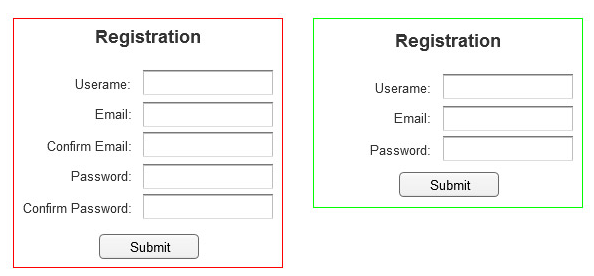
\includegraphics[width=0.6\textwidth]{figuras/account/examples/form_compare.png}

	\caption{Ejemplos de formularios de creación. El formulario de la izquierda pide confirmación de \email y contraseña, implicando en un mayor número de campos a llenar.}
	\label{figure:account:create_account:form_compare}
\end{figure}

Este estilo de creación de cuenta está actualmente implementando en sitios populares como \twitterNAME, \dropboxNAME, \netflixNAME \instagramNAME y \linkedInNAME. Los formularios se pueden ver en las Figuras \ref{figure:apendice:account:example:twitter_create_form}, \ref{figure:apendice:account:example:dropbox_create_form}, \ref{figure:apendice:account:example:netflix_create_form}, \ref{figure:apendice:account:example:instagram_create_form} y \ref{figure:apendice:account:example:linkedin_create_form} respectivamente.


Finalmente se presenta el formulario de creación de usuario en la \refFigura{figure:account:create_account:form}.
\begin{figure}[H]
	\centering
	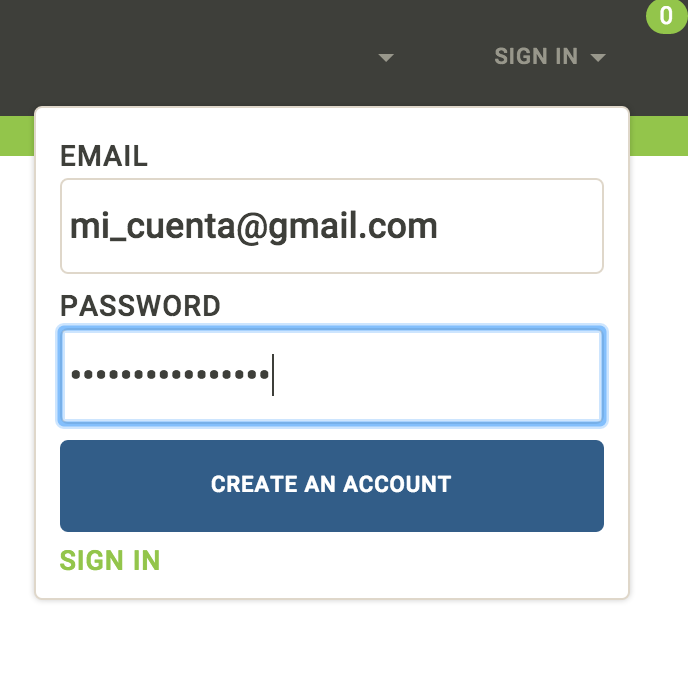
\includegraphics[width=0.4\textwidth]{figuras/architecture/accounts/new/form.png}

	\caption{Formulario de creación de una cuenta.}
	\label{figure:account:create_account:form}
\end{figure}



El formulario de creación tiene ciertas restricciones, las cuales deben cumplirse para la creación exitosa de una cuenta. La \reftabla{tab:architecture:accounts:new:form} resume todas las restricciones del formulario. En la \refFigura{figure:architecture:accounts:new:send_error} pueden verse los errores que muestra el formulario para guiar al usuario.

\begin{table}[H]
    \centering
	\begin{tabular}{ |l|c||l| }
		\hline Campo & Requerido & Restricción \\ \hline
		\multirow{2}{*}{\textit{Email Address}} &  \multirow{2}{*}{\checkmark}
				& - Debe ser un \email válido. \\ 
			& 	& - El \email no debe pertenecer a un usuario previamente ingresado.\\ \hline
		\multirow{2}{*}{\textit{Password}} 		&  \multirow{2}{*}{\checkmark}	
				& - Debe tener al menos 8 caracteres. \\ 
			& 	& - Debe contener al menos un número o símbolo. \\ \hline
	\end{tabular}
 	\caption{Resumen de restricciones para formulario creación de cuentas de usuario.}
    \label{tab:architecture:accounts:new:form}
\end{table}

\subsection{Autenticarse}

Al igual que el formulario de creación de usuario, el formulario de autenticación tiene solo dos campos (\refFigura{figure:account:signin:form}).

\begin{figure}[H]
	\centering
	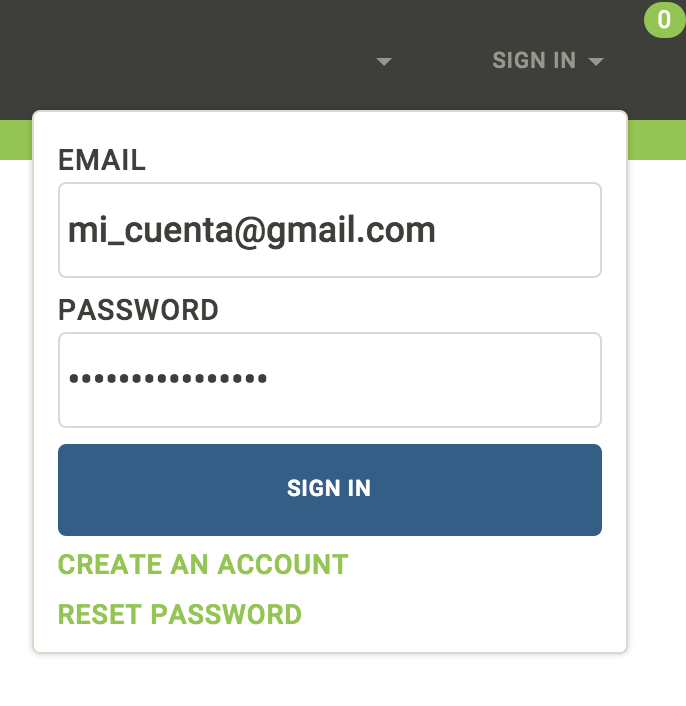
\includegraphics[width=0.4\textwidth]{figuras/architecture/accounts/signin/form.png}
	\caption{Formulario de autenticación en la aplicación.}
	\label{figure:account:signin:form}
\end{figure}

Las restricciones del formulario de autenticación pueden observarse en la \reftabla{tab:architecture:accounts:signin:form}. Un formulario con errores puede verse en \refFigura{figure:architecture:accounts:signin:send_empty}.

\begin{table}[H]
    \centering
	\begin{tabular}{ |l|c||l| }
		\hline Campo & Requerido & Restricción \\ \hline
		\multirow{2}{*}{\textit{Email Address}} &  \multirow{2}{*}{\checkmark}
				& - Debe ser un \email válido. \\ 
			& 	& - El \email debe estar en la base de datos. \\ \hline
		\multirow{1}{*}{\textit{Password}} 		&  \multirow{1}{*}{\checkmark} & - Debe corresponder al \email. \\ \hline
	\end{tabular}
 	\caption{Resumen de restricciones para formulario de autenticación de usuario.}
    \label{tab:architecture:accounts:signin:form}
\end{table}

\subsection{Cerrar sesión}

Una vez autenticado, el formulario de autenticación desaparecerá y en su lugar habrá un botón para cerrar sesión (\refFigura{figure:accounts:logout:form}).

\begin{figure}[H]
	\centering
	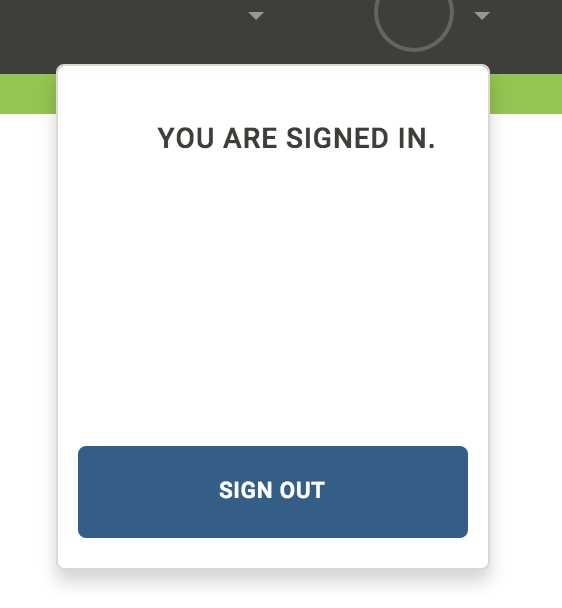
\includegraphics[width=0.4\textwidth]{figuras/architecture/accounts/logout/ui.png}
	\caption{Desvincular la cuenta de la aplicación.}
	\label{figure:accounts:logout:form}
\end{figure}

\subsection{Recuperar contraseña}
Olvidar las contraseñas es algo recurrente. De hecho, más del 81\% ha olvidado una contraseña utilizada en un sitio web \cite{online_berkeley_behavior_toward_password}. Esto demuestra lo importante que es contar con mecanismos de recuperación de contraseña.
El procedimiento es muy sencillo; se envía el \email usando el formulario de recuperación de contraseña (\refFigura{figure:account:reset:form}). El sitio genera una contraseña temporal y es enviada al correo.

\begin{figure}[H]
	\centering
	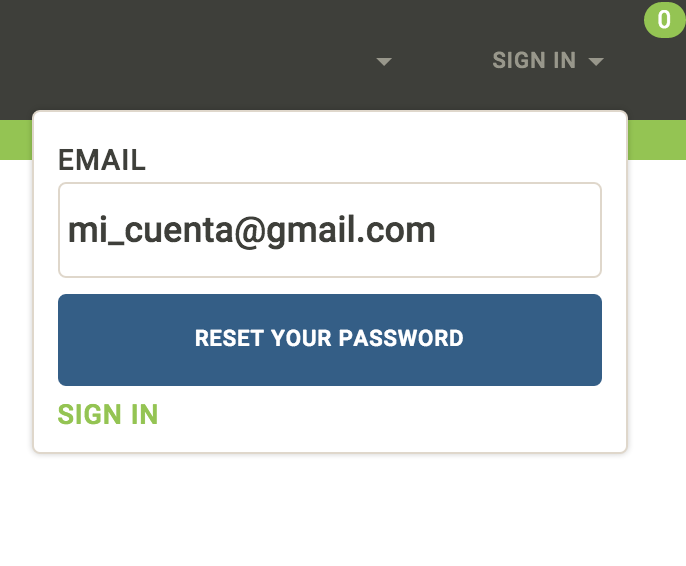
\includegraphics[width=0.4\textwidth]{figuras/architecture/accounts/reset/form.png}
	\caption{Formulario de restauración de contraseña.}
	\label{figure:account:reset:form}
\end{figure}

Las restricciones del formulario de recuperación de contraseña se ven en la \reftabla{tab:architecture:accounts:recovery:form}.

\begin{table}[H]
    \centering
	\begin{tabular}{ |l|c||l| }
		\hline Campo & Requerido & Restricción \\ \hline
		\multirow{2}{*}{\textit{Email Address}} &  \multirow{2}{*}{\checkmark}
				& - Debe ser un \email válido. \\ 
			& 	& - El \email debe estar en la base de datos. \\ \hline
	\end{tabular}
 	\caption{Resumen de restricciones para recuperación de contraseña.}
    \label{tab:architecture:accounts:recovery:form}
\end{table}

\subsection{\loginUpperCPT  con servicio de autenticación \thirdParty}
%\subsection{Autenticarse con proveedores de \oauthLoginINT }

La aplicación permite hacer \loginCPT a través de servicios de autenticación \thirdParty, tales como \facebook, \googleNAME, \twitterNAME, \gitHubNAME, entre otros. En la \refFigura{figure:account:login:log_in_plus_facebook} se observa la existencia de un servicio \thirdParty para la autenticación en la aplicación.


\begin{figure}[H]
	\centering
	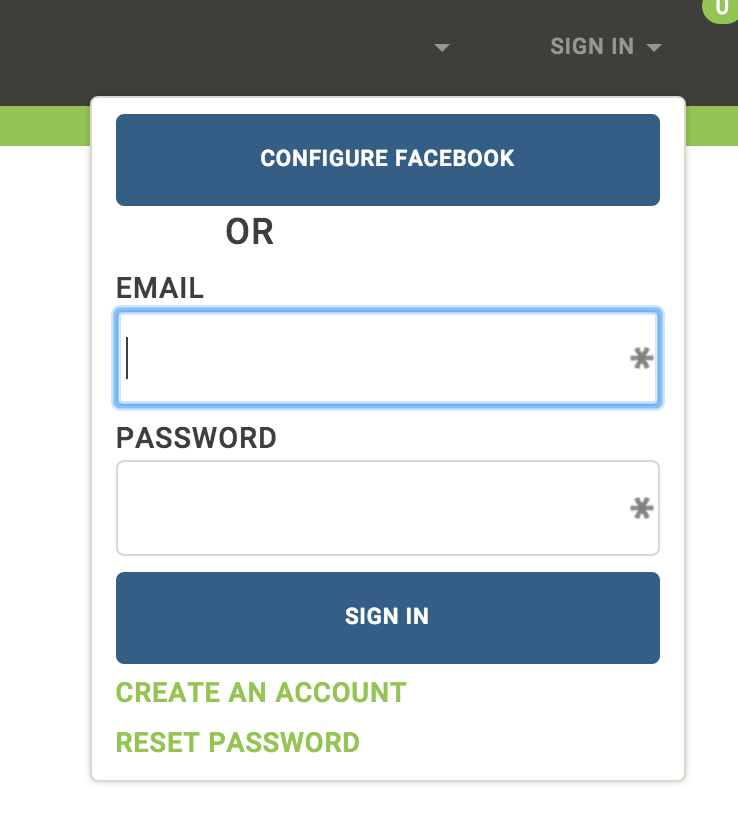
\includegraphics[width=0.4\textwidth]{figuras/architecture/accounts/login/log_in_plus_facebook.png}

	\caption{La aplicación ofrece autenticarse utilizando un servicio \thirdParty (\facebook) o directamente en el sitio.}
	\label{figure:account:login:log_in_plus_facebook}
\end{figure}

Si se hace click sobre el botón \facebook de la \refFigura{figure:account:login:log_in_plus_facebook}, la aplicación irá a una página de \facebook y mostrará el formulario para autenticarse.

%Es importante agregar que el sistema automáticamente agrega en la interfaz la opción de autenticarse utilizando el servicio \thirdParty simplemente agregando el \packagesAS de \meteorNAME; y por consiguiente este desaparecerá si el \packagesAS es removido. En la \refFigura{figure:architecture:accounts:login:log_in_all_package} se aprecian varios servicios \thirdParty para la autenticación de la aplicación.
Es importante destacar que el sistema permite agregar o esconder las opciones \thirdParty de la interfaz. En la \refFigura{figure:architecture:accounts:login:log_in_all_package} se ven los proveedores \oauthLoginINT \facebook, \gitHubNAME, \googleNAME, \twitterNAME, respectivamente. Cada uno de estos botonos enviara la aplicación a autenticarse en su respectivo sitio oficial.

\begin{figure}[H]
	\centering
	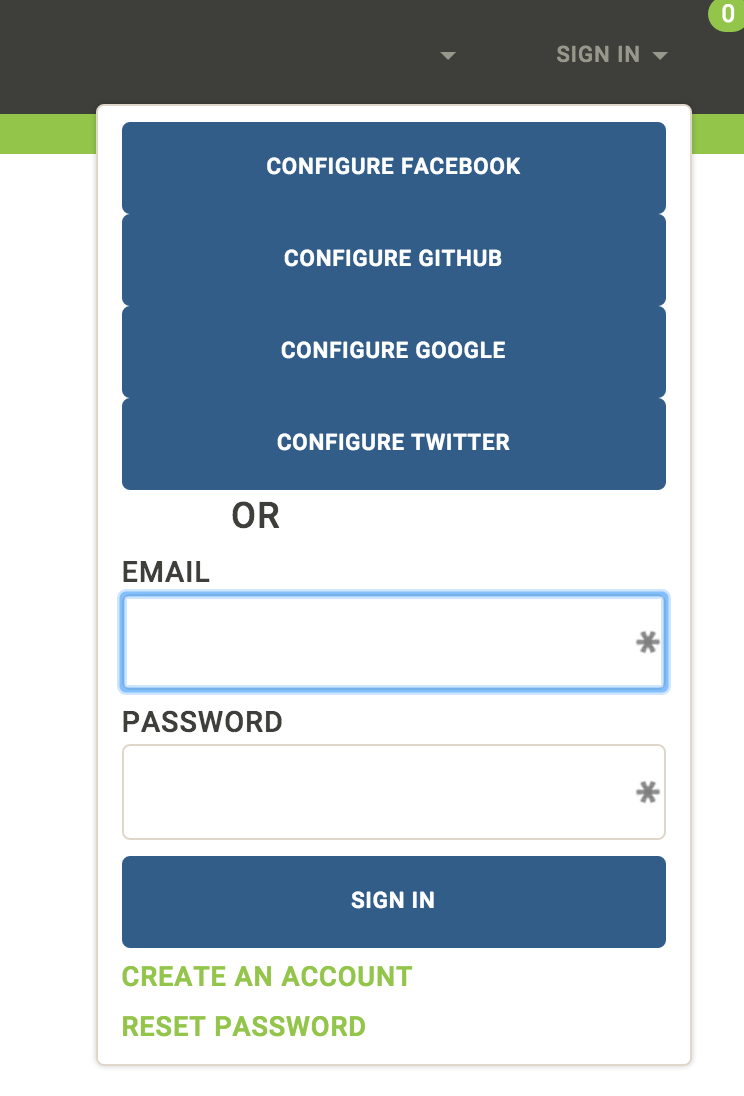
\includegraphics[width=0.4\textwidth]{figuras/architecture/accounts/login/log_in_all_package.png}

	\caption{Formulario de autenticación para utilizar uno de varios servicios \thirdParty.}
	\label{figure:architecture:accounts:login:log_in_all_package}
\end{figure}

% caracteristicas actuales en funcionamiento
%!TEX root = ../../../memoria.tex

%you can provide your own UI for these features or you can even use a premade boilerplate UI to get up and running quickly.

%eteor Accounts is a modular system, and anyone can write a package that provides a new login method. Some, but not all of these packages are officially maintained by the Meteor Project. For example, accounts-password has a complete password-based login system, including password recovery. Packages such as accounts-google, accounts-facebook, and accounts-twitter provide the ability to log in with common third-party authentication services.

%The account database is stored in a users database collection that is automatically created on the server. Currently this can only be stored in MongoDB, but other databases will likely be supported in the future, depending on demand. The schema of this database is shown in the main Meteor docs.

%Passwords are safely encoded with bcrypt according to industry best practices.

\section{Localización}

El inglés no solo ostenta el primer lugar como el idioma más utilizado, \rankingCPT que considera además del porcentaje de población, la distribución geográfica, sino que además es el idioma más usado en los \websitesINT alcanzando la cifra de 59,4\%, seguido tímidamente por Rusia con un 5,9\% \cite{online_world_wide_languages}. Mirando estas cifras se podría concluir que la inclusión de múltiples idiomas en un \siteINT \ecommerceCOM	no reprensentaría ingresos importantes.
El potencial económico \online es de \$45 trillones, de acuerdo a un estudio realizado por \commonSenseAdvisoryNAME \cite{online_world_global_oportunity_multi_languages}.  Sin una sólida estrategia de localización que considere \websitesINT \ecommerceCOM con \textit{multi-idiomas}, será  un desafío tener al alcance de la mano ese \revenueCOM. De hecho, el mismo estudio vislumbró que si solo se tiene una versión en inglés del \siteINT, se estará limitado solo a una tercera parte del total.

%Grow revenue with website localization
%The economic potential of online communication is $45 trillion, according to a recent study by Common Sense Advisory. How exciting! The sky is the limit for your global business.
%Or is it?
%Without a solid localization strategy that incorporates an e-commerce website in multiple languages, it will be a challenge to get within arm’s reach of this revenue. In fact, the same study found that if you have just an English version of your website, you’re limited to only one third of the pot.

¿Cuántos serán los idiomas necesarios para permanecer competitivo en el mundo \online?. Los investigadores dicen que un mínimo de 14. Las marcar mundiales que aspiran a un 95\% de las billeteras \online necesitan de 20 idiomas. Si bien es cierto no es siempre posible mantener contenido \online en 20 idiomas, es difícil negar los beneficios de la localización para regiones específicas alrededor del mundo \cite{online_world_global_oportunity_multi_languages}. Estas son las razones de por qué se considera muy importante la localización en el \frameworkPC y de por qué se aborda esta característica desde los inicios.

Actualmente la aplicación cuenta con un sistema robusto para la localización, permitiendo nuevos idiomas simplemente agregando un archivo \jsonNAME (\refFigura{figure:features:languages_available}).
%How many languages does it take for global businesses to stay competitive online? The research says a minimum of 14. Global brands wanting to appeal to 95 percent of the world’s online wallet need 20 languages. While it isn’t always feasible for a business to translate online content into 20 languages, it’s hard to deny the benefits of website localization for targeted regions around the world.
%Many businesses recognize this and plan to add even more languages to their localization strategy in the future. One example is European-based clothing seller ASOS. They launched a website for the Chinese and Russian markets in 2013 to expand their global footprint. They already had a presence in the United Kingdom, United States, France, Germany and Australia. They saw international sales overall increase by 39 percent with their past website localization initiatives—so they knew that additional language sites would help grow revenue.
%If you’re ready to get a bigger piece of the global e-commerce pie, like ASOS, consider upping the number of languages on your website. Check out the article, Global e-commerce: Are these 5 items in your localization shopping cart?, for tips on how to approach e-commerce website localization.


\begin{figure}[H]
	\centering
	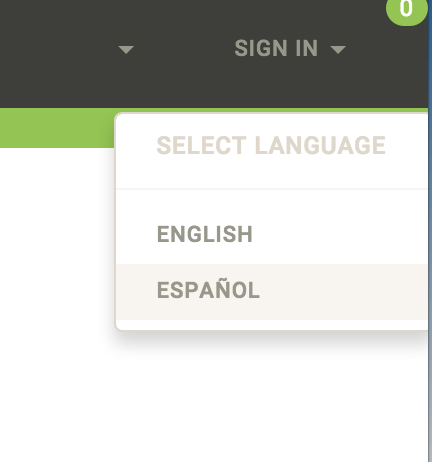
\includegraphics[width=0.3\textwidth]{figuras/languages_available.png}

	\caption{Selección de idioma para el \websiteINT.}
	\label{figure:features:languages_available}
\end{figure}


\section{\themesCPT}

Como se explicó en la subsección \ref{chapter:section:subsection:package_core_theme}, la aplicación permite cambiar el \themeCPT utilizando el \packageAS correspondiente.
Una de las partes más importantes del \frameworkPC \ecommerceCOM corresponde justamente a la customización de la aplicación, dado que esto logra generar identidad.
Posteriormente el sistema permitirá además agregar \templatesAS que permitan una personalizaciónn del \websiteINT aun más detallada.



\section{La información persiste}

Aunque se cambie de vista, al regresar regreso, la información debería seguir viéndose. Por ejemplo, al llenar un formulario  y dejar la página, al regresar, este formulario estará igual.


%TODO: ver si es necesario agregar esto
% caracteristicas actuales en formularios
%%!TEX root = ../../../memoria.tex
\section{Interfaz de Usuario}

Este proyecto no tiene entre sus objetivos la usabilidad de sus interfaces, razón por la cual no es necesario presentar resultados de experiencia de usuario en esta materia, sin embargo, una buena interfaz de usuario se considera buena si tiene un alto \conversionRateCOM y es \textit{fácil de usar} \cite{online_goodgui_org}


% caracteristicas actuales en formularios
%!TEX root = ../../../../../memoria.tex
\section{Formularios}

Los formularios son parte relevante de la aplicación. Por lo tanto se puse especial énfasis en 

\subsection{Pocos campos en los formularios}
Cada uno de los formularios que existen en la aplicación fueron creados con este principio. Los seres humanos son intrínsecamente resistentes a labores de tareas intensivas y el mismo principio se aplica para llenar completamente un formulario. Por cada campo agregado al formulario, se corre el riesgo de perder un cliente\cite{online_goodgui_org}.
%TODO : Agregar referencia a figura de creación de usuario
Un caso claro de esto, corresponde a la interfaz de creación de un usuario ( \refFigura{}), la cual fue diseñada solo con dos campos.


\subsection{Errores}
Los errores ocurriran sin importar las medidas que se tomen. Lo importante es evitar al máximo que estos sucedan. Y cuando esto pase, guiar adecuadamente al usuario para que pueda resolver los problemas sin mayores inconvenientes. Para estos casos se debe proceder de la manera siguiente:
\begin{itemize}
	\item Comunicar claramente que es aquello que esta sucediendo.
	\item Describir como el usuario puede resolverlo.
	\item Mantener tanto \inputBrowserINT del usuario como sea posible \cite{online_google_ui_pattern_error}.
\end{itemize} 


\begin{figure}[H]
	\centering
	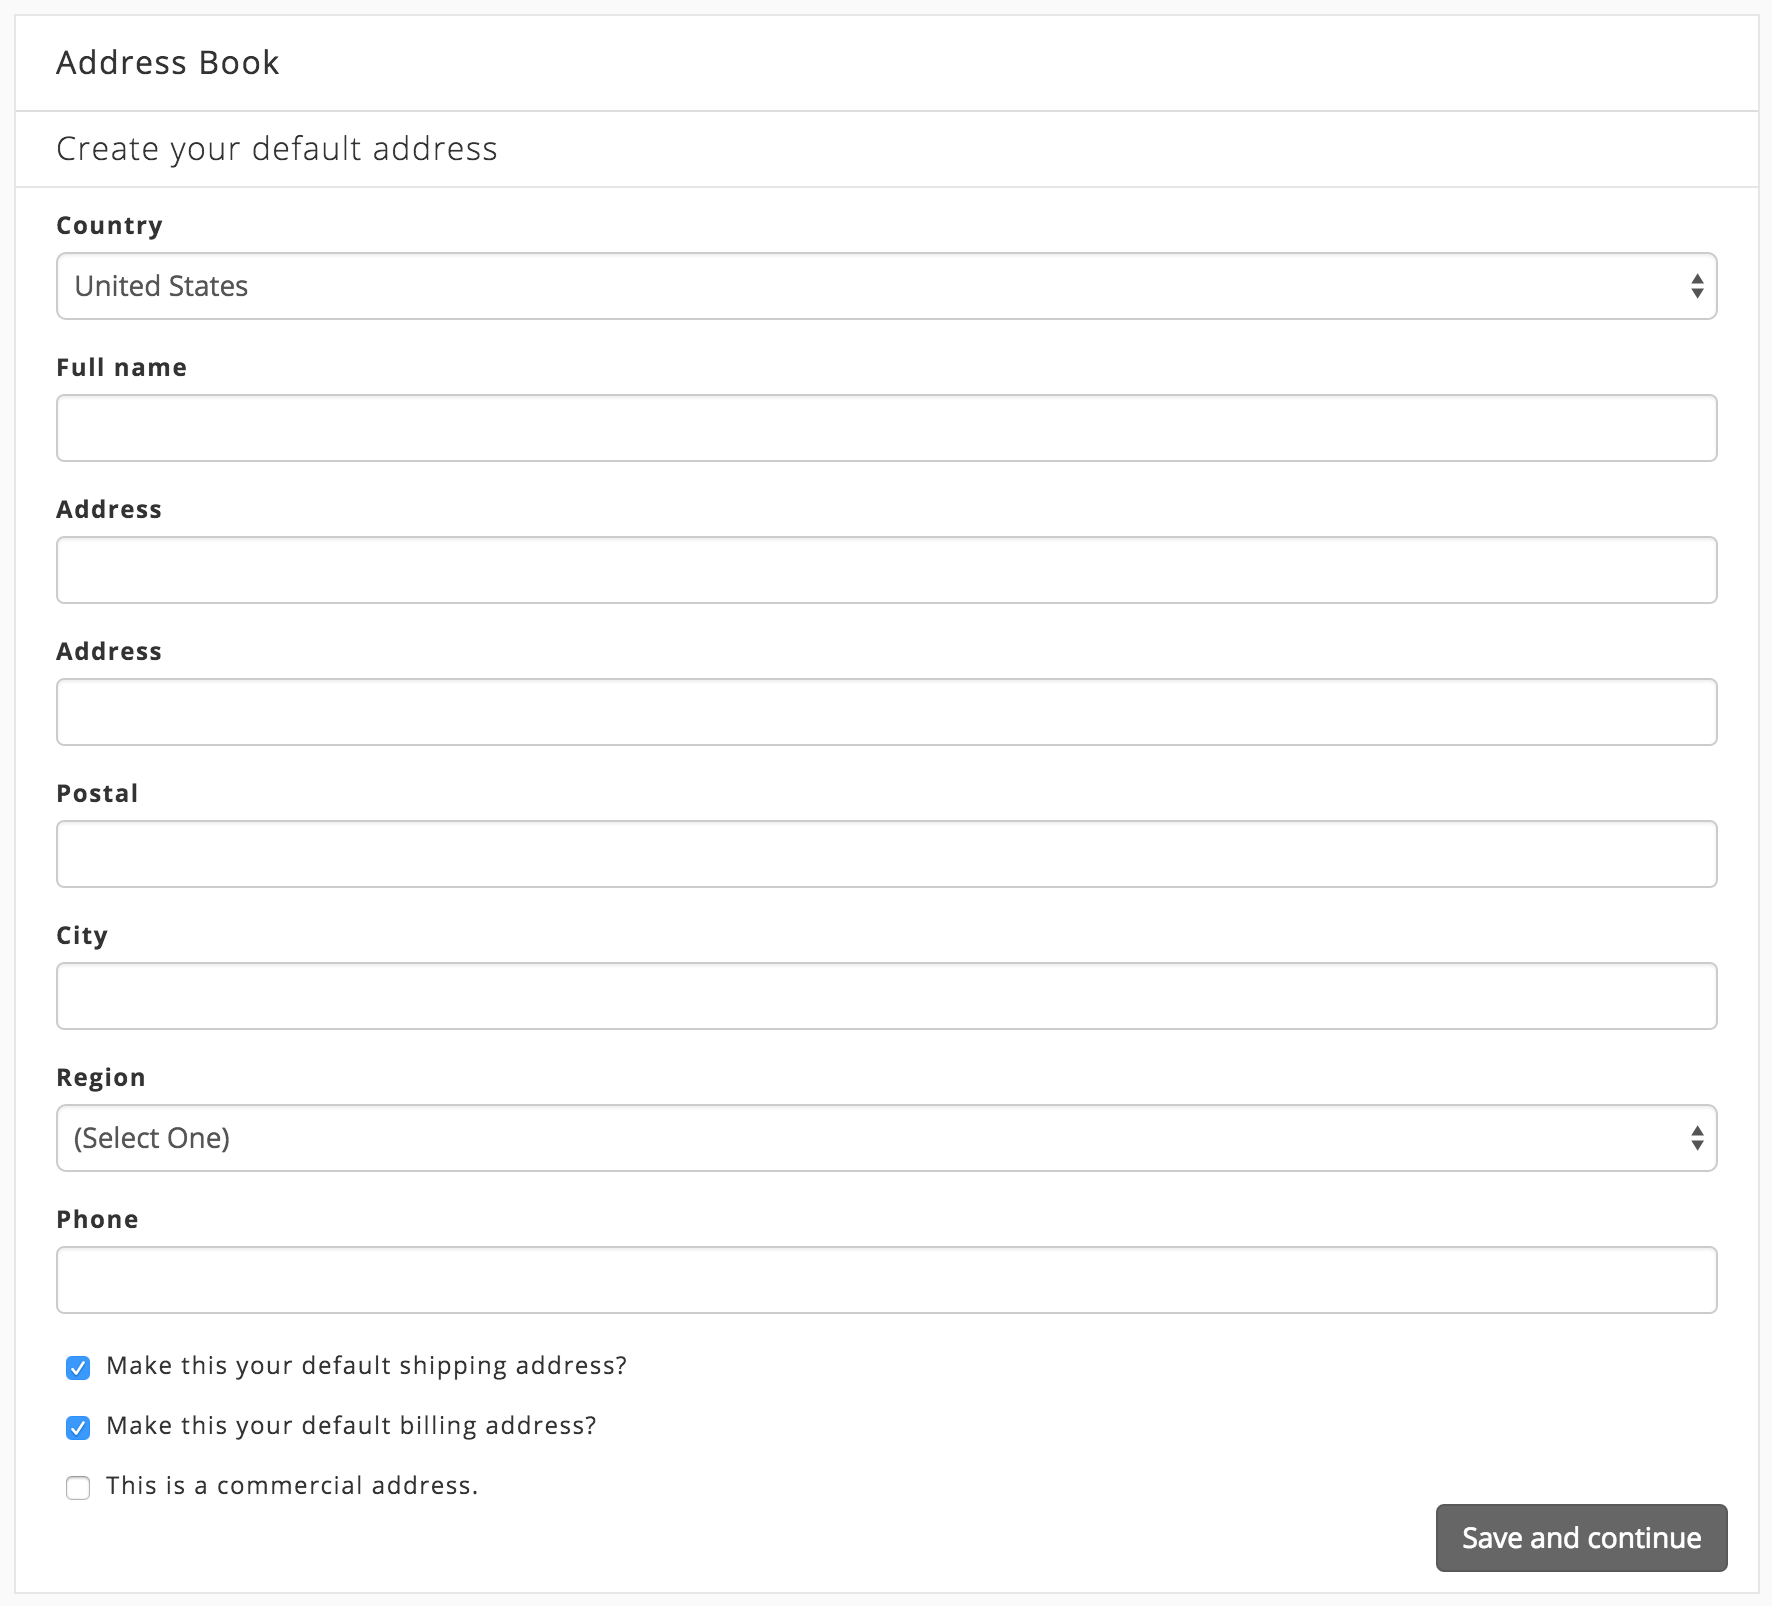
\includegraphics[width=0.5\textwidth]{figuras/formularios/form_address_book.png}

	\caption{Formulario de creación de una nueva dirección de envio.}
	\label{figure:form:form_address_book}
\end{figure}


















% caracteristicas actuales del producto
%!TEX root = ../../../memoria.tex

\section{Productos}

	\subsection{Vista global de productos}\label{chapter:section:productos:subsection:vista_global}
		La interfaz inicial de la aplicación corresponde a la vista de todos los productos que el sistema tiene. En la \refFigura{figure:solution:product:global_view:view} se pueden observar 4 productos.

		\begin{figure}[H]
			\centering
			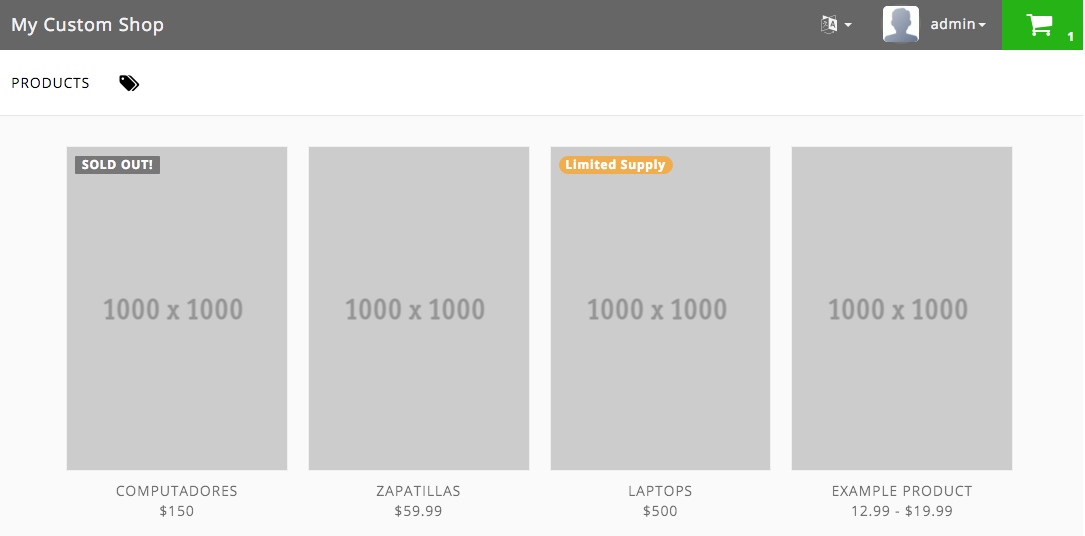
\includegraphics[width=0.8\textwidth]{figuras/solution/product/global_view/view.png}

			\caption{Vista global de los productos. Productos con problemas de \stock dan información.}
			\label{figure:solution:product:global_view:view}
		\end{figure}

		De la interfaz, se observa que hay un producto \textit{SOLD OUT!} y otro producto \textit{LIMITED SUPPLY}. Esto ocurre por que la plataforma tiene un sistema de \trackingCPT de productos la cual puede ser modificada desde la vista \nameref{chapter:section:productos:subsection:edicion}.


		Esta vista depende de los permisos que el usuario que ha ingresado tiene. Si el usuario tiene permisos de edición de productos, tendra la posibilidad de ver todos los productos que existen en el sistema, incluso esos que no estan publicados. En el caso de un usaurio sin permisos de edición, solo tendrá visibilidad de aquellos productos que han sido publicados.

	\subsection{Descripción de un producto}\label{chapter:section:productos:subsection:descripcion}

		La aplicación permite consultar la descripción de un producto. Dicha interfaz puede observarse en la \refFigura{figure:bootstrap:theme_cyborg}. Se puede aprenciar algunas de las carecterísticas de las que ya dispone cada producto.

		\begin{itemize}
			\item
				Un título del producto.
			\item
				Un subtítulo para dar un resumen.
			\item
				Un espacio para la foto del producto.
			\item
				Un lugar para la descripción del producto.
			\item
				Un precio ó intervalo de precios.
		\end{itemize}

	\subsection{Creación de un producto}

		Cuando se penso en la interfaz de creación/edición de un producto, la base era tener una interfaz idéntica a la vista de \nameref{chapter:section:productos:subsection:descripcion}, y por lo tanto, interactuar con los diferentes elementos directamente en la interfaz de vista.
		Cuando se ingresa a la interfaz de vista de un producto con los pemisos adecuados, todas las componenetes de la vista del producto se vuelven componentes editables.

		La interfaz de creación de un producto se observa en la \refFigura{figure:solution:product:create:form}. Es importante destacar la ayuda que brindan los \placeholdersINT para guiar al usuario.

		\begin{figure}[H]
			\centering
			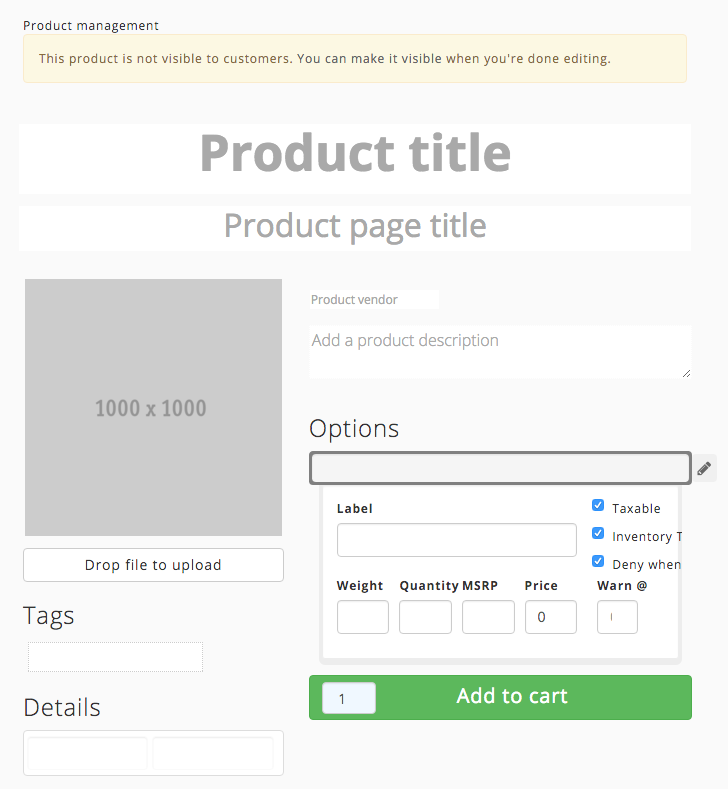
\includegraphics[width=0.8\textwidth]{figuras/solution/product/create/form.png}

			\caption{Interfaz de creación de un producto.}
			\label{figure:solution:product:create:form}
		\end{figure}

		Para determinar los campos utilizados en \refFigura{figure:solution:product:create:form}, de inspiración se utilizó principalmente la interfaz de creación de productos desarollada para el \websiteINT de \shopifyNAME \refFigura{figure:apendice:productos:example:shopify_product_generic_view}. \shopifyNAME es un servicio proporciona toda las herramientas necesarias para desarrollar una tienda \online, razón por la cual cuenta con una gran cantidad de herramientas las cuales no pueden ser avordadas en su totalidad en un contexto de una memoria.
		A continuación se explica cada una de las componenetes utilizadas en el \frameworkPC obtenidas desde  \websiteINT \shopifyNAME:

		\begin{description}
			\item [\titleForm]
				Título principal del producto (\refFigura{figure:product:description:main_tittle}). Idealmente debe ser consiso por que se utiliza tanto en la interfaz de descripción del producto, como en pantalla de búsqueda de productos. El título aparece claramente en la sección principal de la interfaz de creación \refFigura{figure:apendice:productos:example:shopify_product_main}.

				\begin{figure}[H]
					\centering
					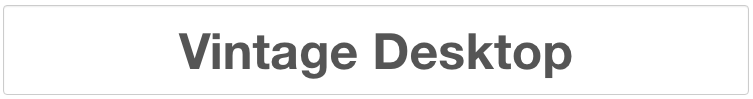
\includegraphics[width=0.6\textwidth]{figuras/product/description/main_tittle.png}

					\caption{Título principal del producto. Aparece también en la lista de búsqueda de productos.}
					\label{figure:product:description:main_tittle}
				\end{figure}

			\item [\pageTitleForm]
				Título exclusivo de la vista \nameref{chapter:section:productos:subsection:descripcion} (\refFigura{figure:product:description:secundary_tittle}). Permite ser más descriptivo que el título. 

				\begin{figure}[H]
					\centering
					\includegraphics[width=0.6\textwidth]{figuras/product/description/secundary_tittle.png}

					\caption{Título secundario del producto. Aparece solo en la página de descripción del producto.}
					\label{figure:product:description:secundary_tittle}
				\end{figure}

			\item [\descriptionForm]
				Permite agregar una descripción del producto(\refFigura{figure:product:description:component_description}). Se encuentra en la sección principal al igual que el \titleForm \refFigura{figure:apendice:productos:example:shopify_product_main}. Esta sección es particularmente importante ( junto con \multimediaForm), por que ayudan en la desición de compra del producto. Es importante agregar descripciones que expliquen el producto, que entreguen \textit{lindas} palabras que fomenten la compra, no una lista de términos técnicos \cite{online_cxpartners_official_people_see_to_buy}.

				\begin{figure}[H]
					\centering
					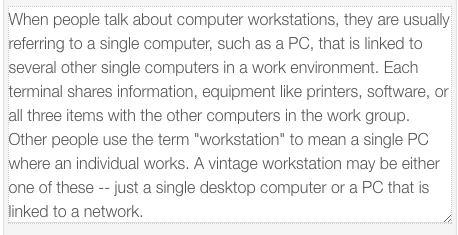
\includegraphics[width=0.6\textwidth]{figuras/product/description/component_description.png}

					\caption{Campo para la descripción del producto.}
					\label{figure:product:description:component_description}
				\end{figure}

			\item [\vendorForm]
				Permite agregar un \vendorForm a la descripción del producto. Aparece en la sección de organización de \shopifyNAME \refFigura{figure:apendice:productos:example:shopify_product_organization}

				\begin{figure}[H]
					\centering
					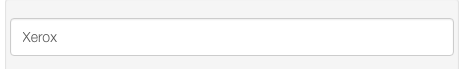
\includegraphics[width=0.6\textwidth]{figuras/product/description/component_vendor.png}

					\caption{Campo para el \vendorForm del producto.}
					\label{figure:product:description:component_vendor}
				\end{figure}

			\item [Options]
				% TODDO : se supone que va aca el \optionsForm
				
			\item [\multimediaForm]
				Al igual como en \shopifyNAME \refFigura{figure:apendice:productos:example:shopify_product_multimedia},esta sección permite agregar imágenes a traves de 2 métodos: \dragdrop y selección utilizando el explorador de archivos \refFigura{figure:product:description:component_multimedia}.
				Las imágenes siempre han sido lo primero que el cliente ve. La mayoria de los \websiteINT ubican las imágenes en la parte superior izquierda de la página \cite{online_cxpartners_official_people_see_to_buy}.
				A diferencia de los compraderos en las tiendas, las imágenes de los productos son la única forma real de determinar si un producto se ajusta a sus necesidades y a sus preferencias. Es una manera poderosa de darle vitrina a los productos. Por lo tanto es muy importante proveer de imágenes de buena calidad entre otros detalles \cite{online_cxpartners_official_people_see_to_buy}. Esto explica el tamaño de imagen que se acepta en la plataforma.

				\begin{figure}[H]
					\centering
					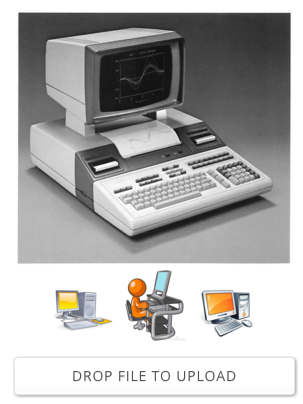
\includegraphics[width=0.6\textwidth]{figuras/product/description/component_multimedia.png}

					\caption{Sección de las imágenes del producto.}
					\label{figure:product:description:component_multimedia}
				\end{figure}
				
			\item [\tagsForm]
				Provenientes de la sección organización \refFigura{figure:apendice:productos:example:shopify_product_organization}, permite la categorización utilisando palabras clave relevantes.

				\begin{figure}[H]
					\centering
					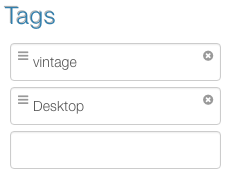
\includegraphics[width=0.6\textwidth]{figuras/product/description/component_tags.png}

					\caption{Campo para las \tagsForm del producto.}
					\label{figure:product:description:component_tags}
				\end{figure}
				
		\end{description}

		También se tuvo en consideración la siguiente información al momento de desarrollar esta interfaz:

		\begin{itemize}
			\item Los visitantes prefieren imágenes de los productos a la izquierda y la descripción a la derecha \cite{online_cxpartners_official_people_see_to_buy}.
			\item Es improbable que un usuario haga \scrollCPT(en el caso de interfaces \desktop) para ver más contenido en la página \cite{online_cxpartners_official_people_see_to_buy}.
			\item Usuarios nunca o muy rara vez leen toda la información disponible especialmente cuando hay muchísimo contenido. Usualmente se ignora la parte inferior o recorren sin poner atención a todas las secciones. E incluso si hacen \scrollCPT, ellos no necesariamente leen o ponen atención a todo el contenido inferior de la página \cite{online_cxpartners_official_people_see_to_buy}.
			%Customers never, or hardly ever read everything you put on the page especially when there is a lot of content! Even if it has a good layout, a long page does not work well. Users often ignore the bottom bits or skim through without paying attention to all sections. And even if they do scroll down, they do not necessarily read or pay attention to all the content below the page.
			\item Agregar solo la información importante del producto que se venderá \cite{online_cxpartners_official_people_see_to_buy}.

			\item Proveer un espació razonable y no sobre utilizar colores \cite{online_cxpartners_official_people_see_to_buy}.

			\item Evitar el uso de \clicking si se desea que el usuario lea \cite{online_cxpartners_official_people_see_to_buy}.
		\end{itemize}


		De los campos que se observan en la \refFigura{figure:solution:product:create:form}: \titleForm, \pageTitleForm, \vendorForm, \descriptionForm, \tagsForm y \detailsForm, tienen \feedbackReactivoDEF. Las restricciones en la creación de un producto se encuentra en la \reftabla{tab:solution:products:create:form:product:generic}. 

		\begin{table}[H]
		    \centering
			\begin{tabular}{ |l|c||l| }
				\hline Campo & Requerido & Restricción \\ \hline
				\multirow{1}{*}{\titleForm} 			&  \multirow{1}{*}{\checkmark} & - Debe tener al menos un caracter. \\ \hline
				\multirow{1}{*}{\pageTitleForm} 	&  \multirow{1}{*}{} &  \\ \hline
				\multirow{1}{*}{\vendorForm}		&  \multirow{1}{*}{} &  \\ \hline
				\multirow{1}{*}{\optionsForm}		&  \multirow{1}{*}{\checkmark} &  \\ \hline
				\multirow{1}{*}{\descriptionForm}	&  \multirow{1}{*}{} &  \\ \hline
				\multirow{1}{*}{\multimediaForm}	&  \multirow{1}{*}{} &  \\ \hline
				\multirow{1}{*}{\tagsForm}			&  \multirow{1}{*}{} &  \\ \hline
				%\multirow{1}{*}{\detailsForm}		&  \multirow{1}{*}{} &  \\ \hline
			\end{tabular}
		 	\caption{Resumen restrincciones para formulario creación de un producto.}
		    \label{tab:solution:products:create:form:product:generic}
		\end{table}

		Como se aprecia en la \reftabla{tab:solution:products:create:form:product:generic}, el campo \detailsForm no es requerido, sin embargo, cada \detailForm en realidad es un objeto compuesto cuyos campos si son obligatorios(\reftabla{tab:solution:products:create:form:product:generic:details}).

		\begin{table}[H]
		    \centering
			\begin{tabular}{ |l|c||l| }
				\hline Campo & Requerido & Restricción \\ \hline
				\multirow{1}{*}{\textit{Anónimo key}}	&  \multirow{1}{*}{\checkmark} & - Debe tener al menos un caracter. \\ \hline
				\multirow{1}{*}{\textit{Anónimo Value}}	&  \multirow{1}{*}{\checkmark} & - Debe tener al menos un caracter. \\ \hline
			\end{tabular}
		 	\caption{Resumen restrincciones para formulario creación de \detailsForm.}
		    \label{tab:solution:products:create:form:product:generic:details}
		\end{table}

		Si no enfocamos en los campos de la \refFigura{figure:product:description:product_options} se observa que ellos se encuentran repartidos entre las secciones \PricingForm(\refFigura{figure:apendice:productos:example:shopify_product_princing}), \InventoryForm(\refFigura{figure:apendice:productos:example:shopify_product_inventory}), \ShippingForm(\refFigura{figure:apendice:productos:example:shopify_product_shipping}) y \VariantsForm(\refFigura{figure:apendice:productos:example:shopify_product_variant_max}).

		\begin{description}
			\item [\LabelForm]
				Corresponde al nombre de la \VariantsForm del producto que se utiliza.

			\item [\OptionForm]
				Se utiliza para identificar cada una de las \VariantsForm al momento de agregarlas al carro.

			\item [\WeightForm]
				Corresponde al peso (masa), del producto que se esta ofreciendo. Este valor se utiliza para \shipping, razón por la cual aparece esta componente en la sección \ShippingForm del formulario de \shopifyNAME \refFigura{figure:apendice:productos:example:shopify_product_shipping}.

			\item [\trackingForm]
				Permite tomar acciones dependiendo del inventario que se tenga. Ver \refFigura{figure:apendice:productos:example:shopify_product_inventory}.

			\item [\denyForm]
				Al igual que el la sección \InventoryForm de \shopifyNAME(\refFigura{figure:apendice:productos:example:shopify_product_inventory}), esta componente aparece cuando se ha seleccionado la opción de \trackingForm. Esta opción evita que los clientes sigan comprando el producto una vez que se ha terminado el inventario.

			\item [\taxableForm]
				Aplica Cargos de impuesto al producto.

			\item [\quantityForm]
				Cantidad de elementos para este producto en particular.

			\item [\priceForm]
				Precio de este producto en particular.
		\end{description}

		\begin{figure}[H]
			\centering
			\includegraphics[width=0.6\textwidth]{figuras/product/description/product_options.png}

			\caption{Sección de las opciones del producto.}
			\label{figure:product:description:product_options}
		\end{figure}

		\begin{table}[H] 
		    \centering
			\begin{tabular}{ |l|c||l| }
				\hline Campo & Requerido & Restricción \\ \hline
				\multirow{1}{*}{\textit{Label}}		&  \multirow{1}{*}{\checkmark} 	& - Debe tener al menos un caracter \\ \hline
				\multirow{1}{*}{\textit{\WeightForm}}	&  \multirow{1}{*}{\checkmark} 	& - Número racional mayor o igual a '0' \\ \hline
				\multirow{1}{*}{\quantityForm}	&  \multirow{1}{*}{\checkmark} 	& - Número entero \\ \hline
				\multirow{1}{*}{\msrpSIGLAS}		&  \multirow{1}{*}{} 			& - Número racional mayor o igual a '0' \\ \hline
				\multirow{1}{*}{\priceForm}		&  \multirow{1}{*}{\checkmark} 	& - Número racional mayor o igual a '0' \\ \hline
				\multirow{1}{*}{\denyForm}		&  \multirow{1}{*}{\checkmark} 	& - Boolean \\ \hline
				\multirow{1}{*}{\warnForm}		&  \multirow{1}{*}{} 			& - Número racional mayor o igual a '0' \\ \hline
				\multirow{1}{*}{\taxableForm}	&  \multirow{1}{*}{\checkmark} 	& - Boolean \\ \hline
				\multirow{1}{*}{\trackingForm}	&  \multirow{1}{*}{\checkmark} 	& - Boolean \\ \hline
			\end{tabular}
		 	\caption{Resumen restrincciones para formulario creación de \optionsForm.}
		    \label{tab:solution:products:create:form:product:generic:options}
		\end{table}

	\subsection{Edición de un producto}\label{chapter:section:productos:subsection:edicion}

		Al igual que para la creación de productos, la edición requiere de permisos especiales. Si se cuenta con dichos permisos especiales, la interfaz de la vista de un producto inmediatamente permite editar los campos. Para editarlos, simplemente es necesario seleccionar la componente con el \mousePC y hacer un \click. La componente cambiara su aspecto para dar \feedback al usuario de que esta seleccionada dicha componente y que puede realizar sobre el ediciones. En la \refFigura{figure:features:interfaz_edicion_editando_description} y \ref{figure:features:interfaz_edicion_editando_subtitulo} es posible apreciar la componentes que se ha seleccionado para editar.

		\begin{figure}[H]
			\centering
			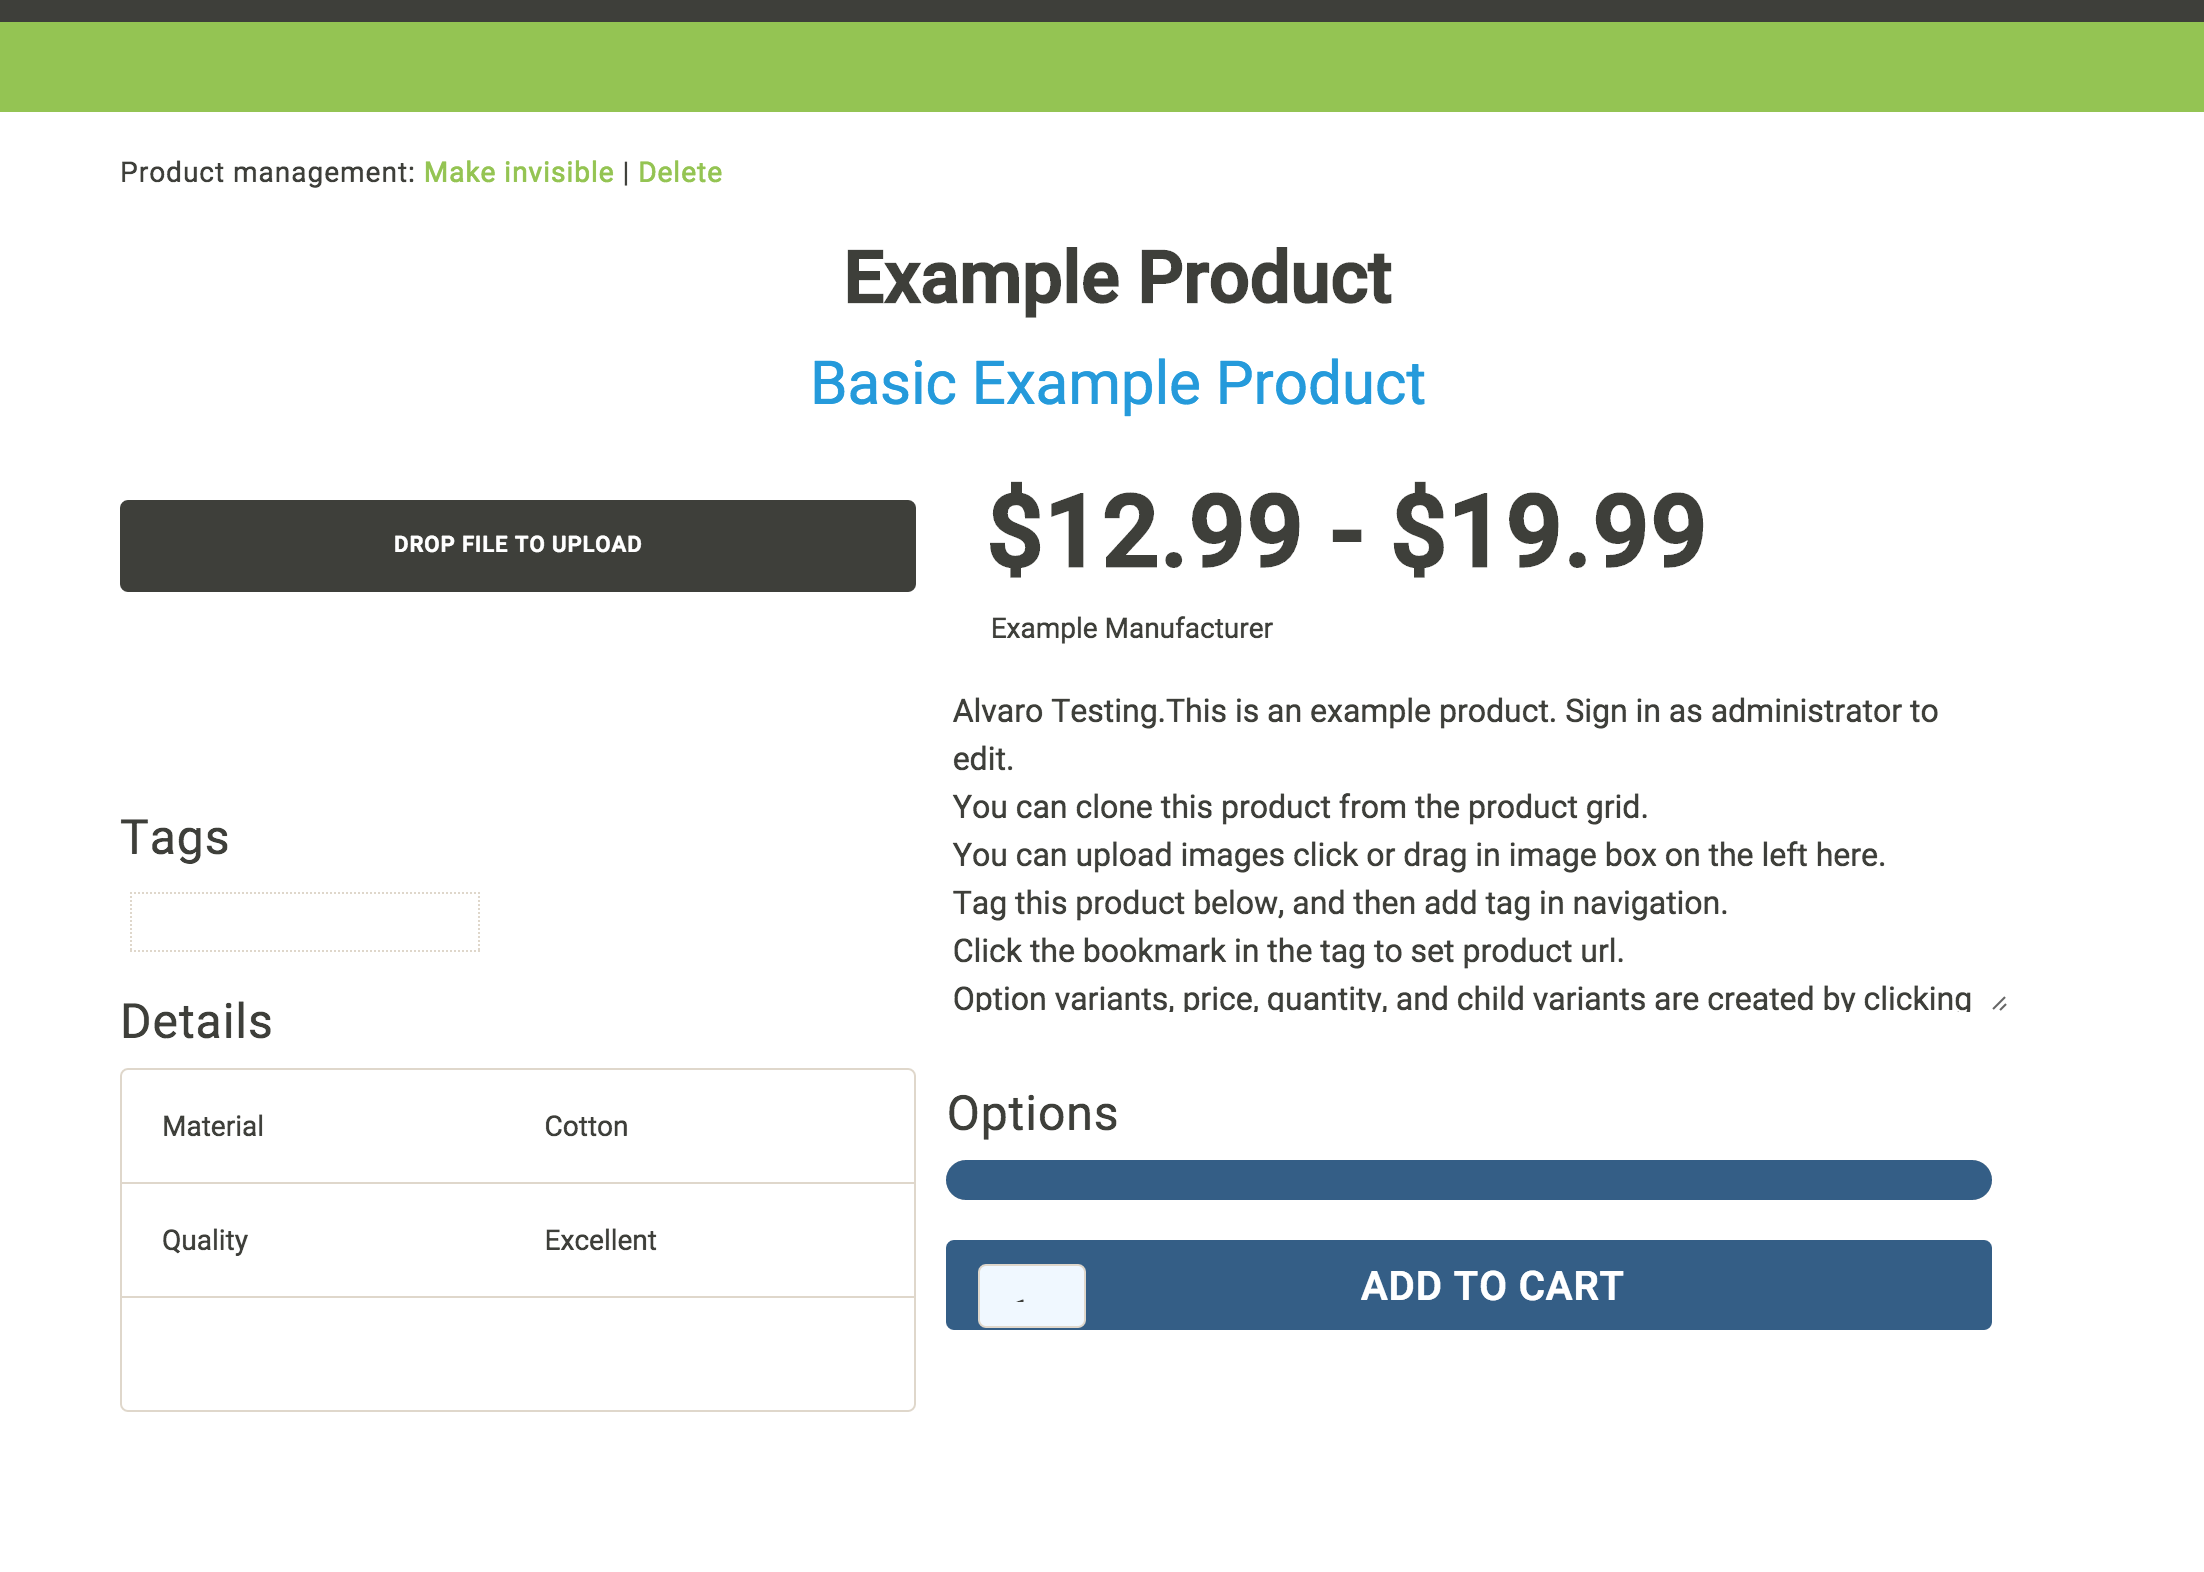
\includegraphics[width=0.8\textwidth]{figuras/productos/interfaz_edicion_producto.png}

			\caption{Interfaz de la edición de un producto.}
			\label{figure:features:interfaz_edicion_producto}
		\end{figure}

		\begin{figure}[H]
			\centering
			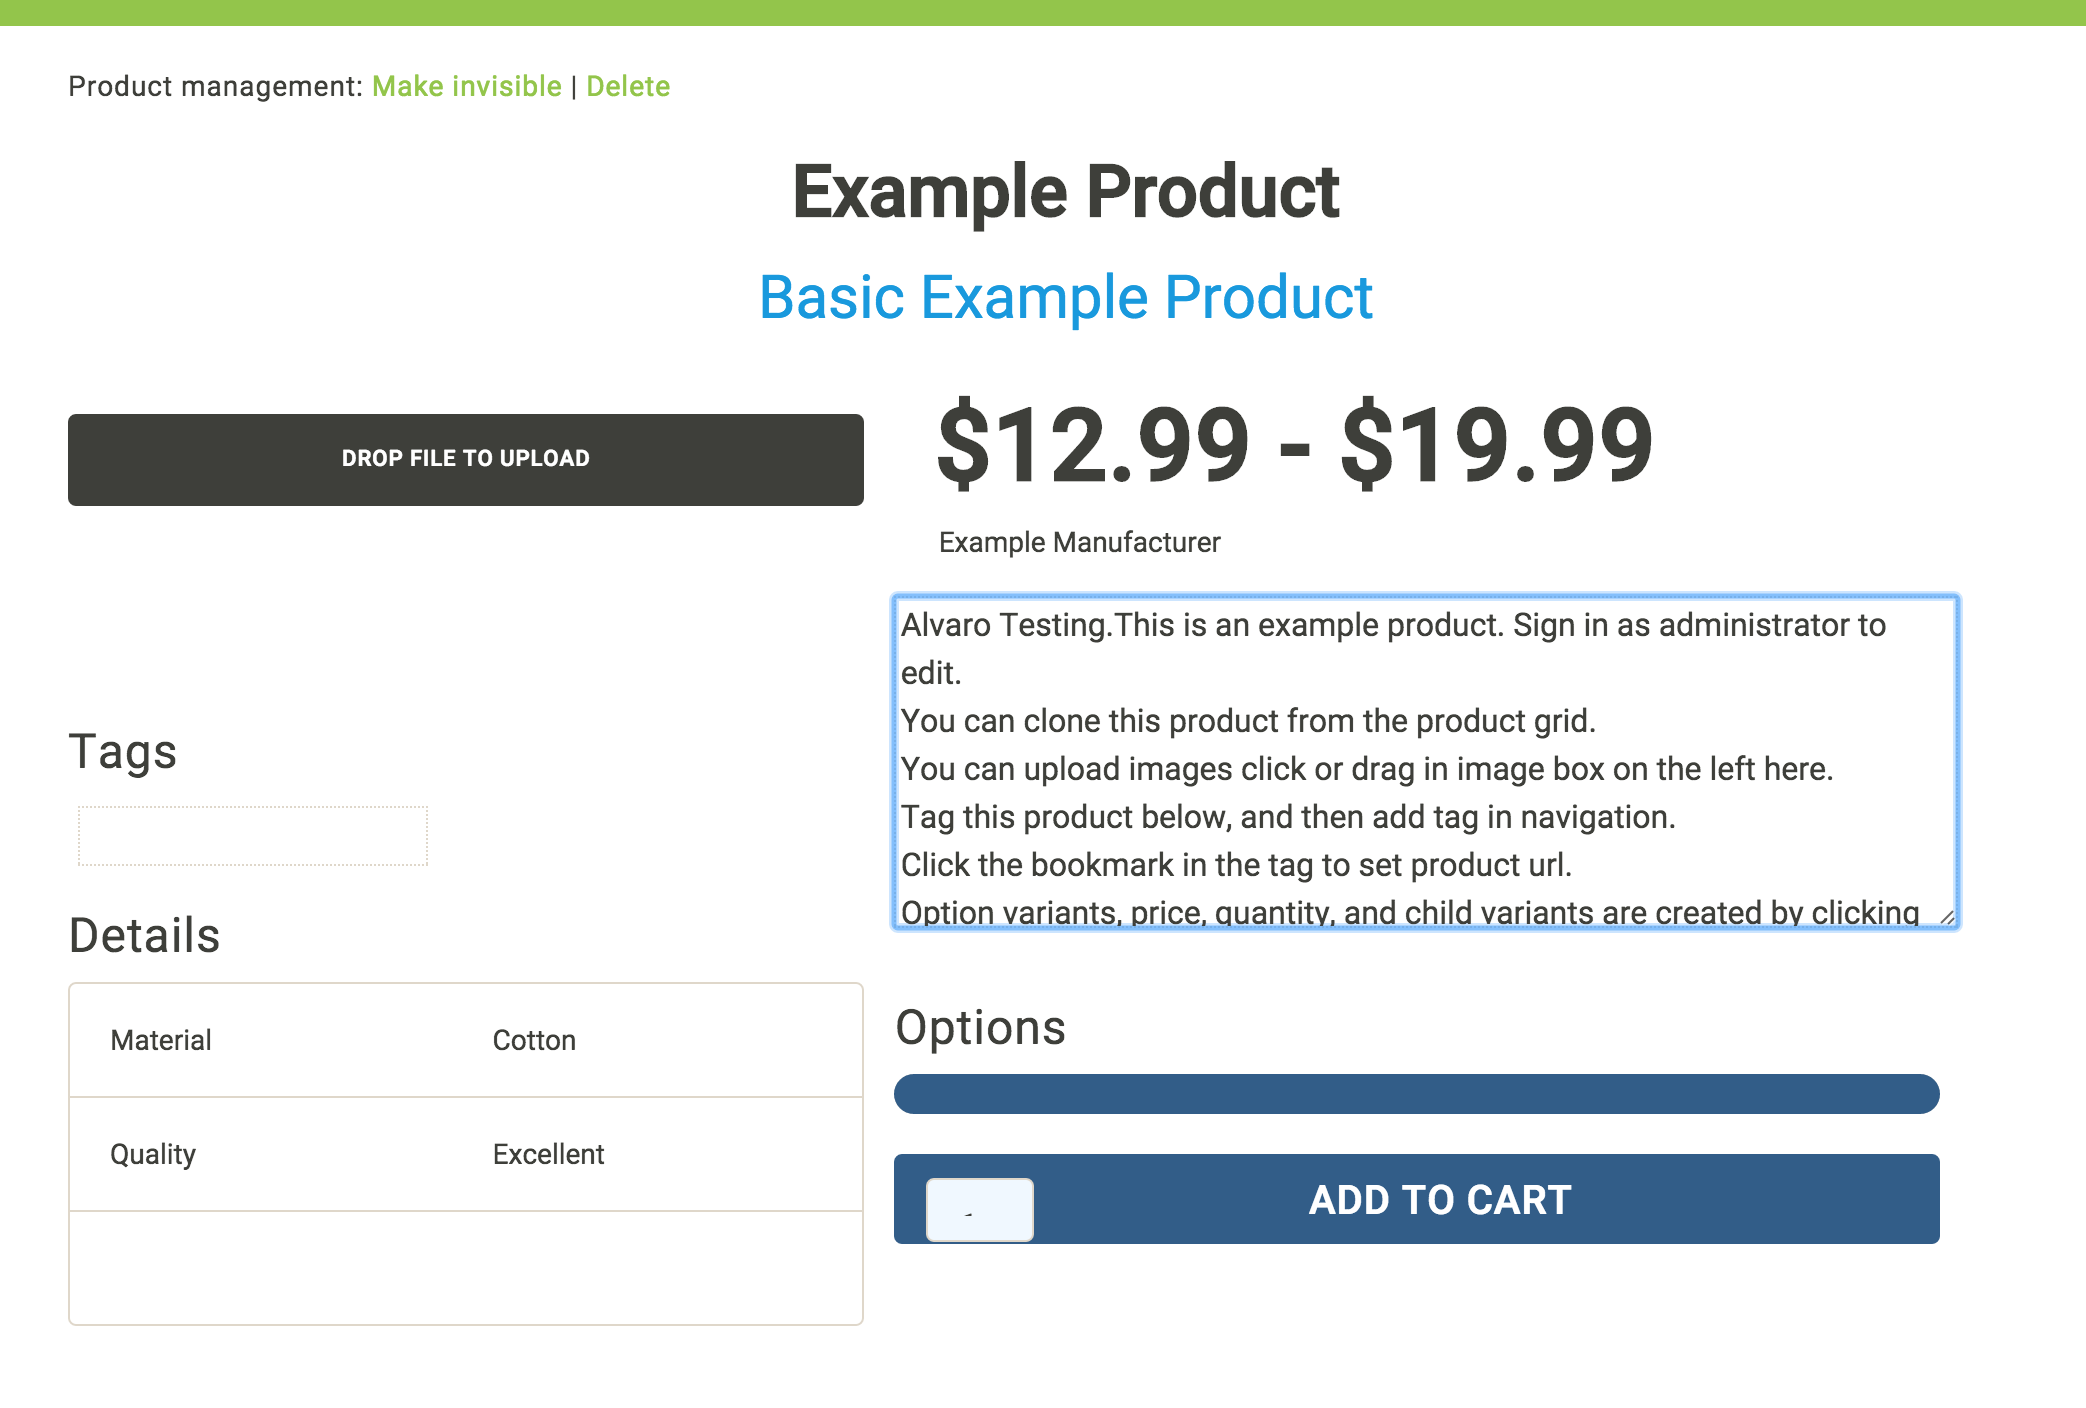
\includegraphics[width=0.8\textwidth]{figuras/productos/interfaz_edicion_editando_description.png}

			\caption{Campo descripción seleccionado para edición.}
			\label{figure:features:interfaz_edicion_editando_description}
		\end{figure}


		\begin{figure}[H]
			\centering
			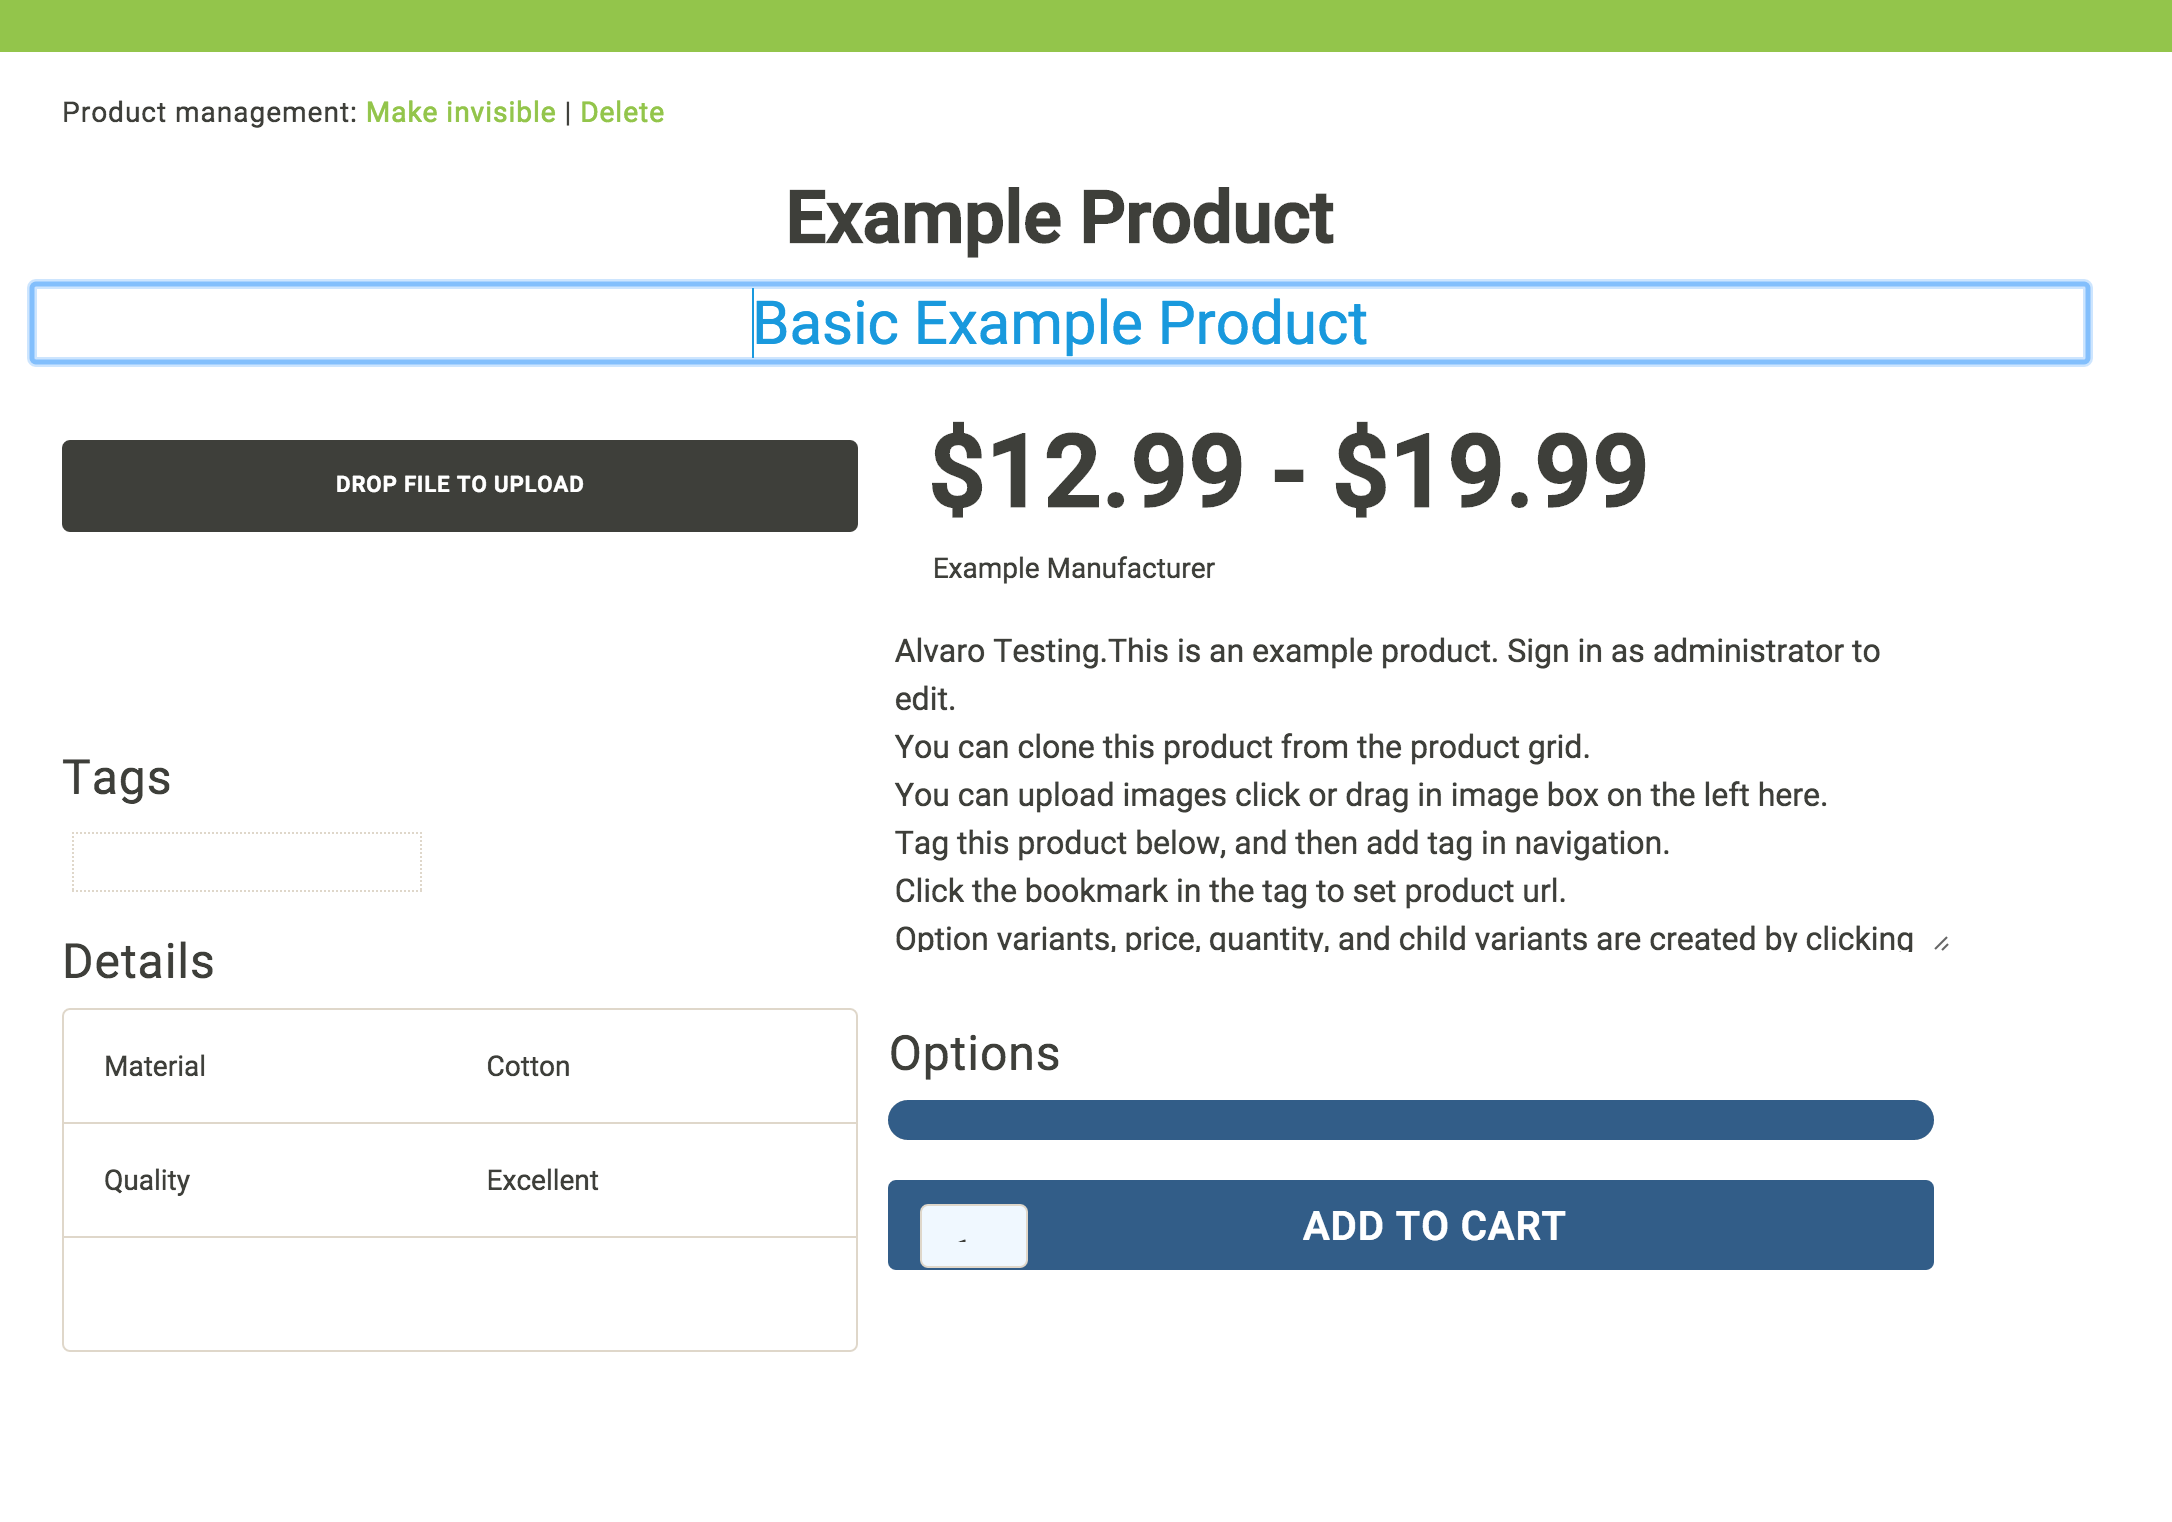
\includegraphics[width=0.8\textwidth]{figuras/productos/interfaz_edicion_editando_subtitulo.png}

			\caption{Campo subtítulo seleccionado para edición.}
			\label{figure:features:interfaz_edicion_editando_subtitulo}
		\end{figure}

		Es importante mencionar que la edición de producto es \reactive, por lo tanto todos los cambios que se realizen serán inmediatamente visibles por parte de todos los usuarios que esten mirando la descripción del producto incluso sin la necesidad de que el usuario haga un \refreshCPT del \websiteINT.

	%TODO: Agregar esta seccion en el futuro
	%\subsection{Eliminación de un producto}

	\subsection{Visibilidad de un producto}
	
		Todo producto válido puede ser visible para todos los usuarios(visibilidad global), o solo visible para aquellos que tienen permiso de edición sobre dicho producto. Esta importante característica se encuentra disponible en el servicio de \shopifyNAME(\refFigura{figure:apendice:productos:example:shopify_product_visibility}). En la \refFigura{figure:solution:product:visibility:new} se ve el caso particular de un producto que esta en proceso de creación (no tiene título, el cual es requerido).

		\begin{figure}[H]
			\centering
			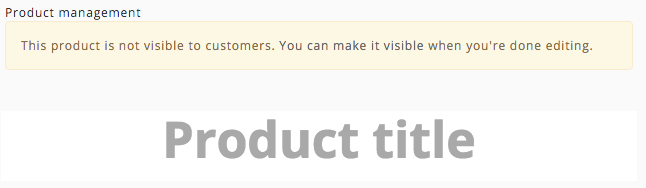
\includegraphics[width=0.8\textwidth]{figuras/solution/product/visibility/new.png}

			\caption{Producto con visibilidad limitada. Notar que no tiene título, lo que implíca que no es un producto válido aún.}
			\label{figure:solution:product:visibility:new}
		\end{figure}

		Después de llenar todos los campos mínimos requeridos para la creación de un producto, es posible presionar el \linkINT \youCanMakeItVisibleLABEL y dar visibilidad global al producto. En el caso que no estén llenos todos los campos requerídos, entonces se generá un \autoFocoINT del primer campo no completado requerido. Suponiendo que se intenta dar visibilidad del producto de la \refFigura{figure:solution:product:visibility:new}, se hara un \autoFocoINT del campo título, el cual puede observarse en la \refFigura{figure:solution:product:visibility:autofocus}; además de mantener el estado de visibilidad (no visible para todos). Esto ocurre para mostrar claramente al usuario que esta sucediendo \cite{online_google_ui_pattern_error,online_goodgui_org}.

		\begin{figure}[H]
			\centering
			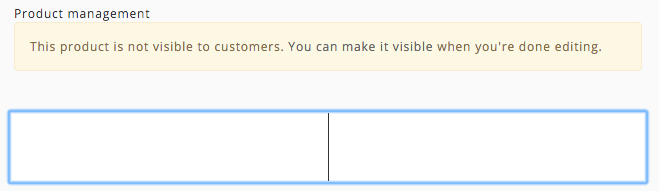
\includegraphics[width=0.8\textwidth]{figuras/solution/product/visibility/autofocus.png}

			\caption{Resultado tras dar visibilidad a un producto sin título. Se genera un \autoFocoINT en el campo título, dado que este es requerido y el estado de visibilidad del producto continua igual.}
			\label{figure:solution:product:visibility:autofocus}
		\end{figure}

		Si todos los campos requeridos de un producto están completos, y se presiona el \linkINT \youCanMakeItVisibleLABEL, se tendra el resultado de la \refFigura{figure:solution:product:visibility:global_visibility}; en donde se observa como el texto superior cambío. Ahora aparece un \linkINT con el texto \makeInvisibleLABEL, para dar \feedback al usuario de lo que ha ocurrido \cite{online_google_ui_design_material,online_goodgui_org}.

		\begin{figure}[H]
			\centering
			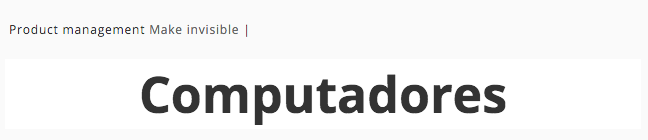
\includegraphics[width=0.8\textwidth]{figuras/solution/product/visibility/global_visibility.png}

			\caption{Producto con visibilidad global. Aparece un \linkINT \makeInvisibleLABEL para ocultar el producto.}
			\label{figure:solution:product:visibility:global_visibility}
		\end{figure}

		%Si se intenta dar visibilidad global de un producto que no esta completo (ver requerimientos de \reftabla{tab:solution:products:create:form:product:generic}), se hará un autofoco al primer elmemento que sea requerido pero que no este completo. Como ejemplo, vemos la \refFigura{figure:solution:product:visibility:new} 	


% caracteristicas actuales en profile
% DONE
%!TEX root = ../../../memoria.tex
\section{Carro Compra}
	El carro de compra agrupa todos los productos seleccionados para efectuar la compra. Actualmente del carro de compra se pueden desprender dos acciones: \nameref{chapter:section:carro_compra:subsection:add} y \nameref{chapter:section:carro_compra:subsection:request}.

	\subsection{Agregar elementos al carro}\label{chapter:section:carro_compra:subsection:add}

		El proceso de agregar elementos es muy sencillo, simplemente hay que ir a la vista de un producto, ir donde esta el botón \addtocartLABEL, seleccionar la cantidad de productos que se desean agregar y finalmente apretar el botón. En la \refFigura{figure:solution:cart:button} se han seleccionado 4 productos para agregar al carro. Este diseño ha sido inspirado también por el \websiteINT de \shopifyNAME (\refFigura{figure:apendice:productos:example:leifshop_product_section_add_to_cart}).

		\begin{figure}[H]
			\centering
			
\includegraphics[width=0.8\textwidth]{figuras/solution/cart/button.png}
			\caption{Botón para agregar productos al carro. En la figura se han seleccionado 4 productos iguales para agregar al carro de compra.}
			\label{figure:solution:cart:button}
		\end{figure}

		Mostrar la confirmación de objeto agregado y permanecer en la misma página es algo fundamental. Las personas no han pedido moverse a otra página, de esta manera no hay sorpresas y se mantiene la buena experiencia. Además es posible que consideren agregar más productos al carro antes de \checkoutCOM \cite{online_official_conversionxl_checkout_flow}. Consideranto esto, se muestra una notificación en la parte superior de la pantalla sobre el ingreso del nuevo producto al carro sin abandonar la página actual (\refFigura{figure:solution:cart:add_motification}).

		\begin{figure}[H]
			\centering
			\includegraphics[width=0.8\textwidth]{figuras/solution/cart/add_motification.png}
			\caption{\FeedbackCPT del nuevo producto agregado al carro.}
			\label{figure:solution:cart:add_motification}
		\end{figure}

		Usualmente el \textit{agregar al carro}, el botón con la acción final \websiteINT \ecommerceCOM cae en una de estas dos opciones: no está bien diseñado o no está ubicado estratégicamente para el uso del cliente \cite{online_official_usabilitygeek_guidelines_usability}. Por esta razón se creó un botón evidente, claro y prominente, en comparación a otras funcionalidades dentro de la misma página. Un ejemplo de lo que no se debe hacer se observa en la \refFigura{figure:apendice:productos:example:usabilitygeek_guidelines_wrong_ui_add_to_cart}.
		%Very often, the ‘Add to Cart’, the final action button in an e-Commerce website is either not well designed or strategically placed to grab prospective buyer’s action. The selection of shape, color, font typography, and button content all trigger the final action. Make sure the ‘Add to Cart’ button is obvious, bright, and prominent in comparison to other features on product page such as wishlists, view product, email to friend, or check out buttons. Less important functions should be lighter colored buttons or simple text links.

		\begin{figure}[H]
			\centering
			
\includegraphics[width=0.3\textwidth]{figuras/productos/examples/usabilitygeek_guidelines_wrong_ui_add_to_cart.png}
			\caption{Mala práctica en el diseño del botón para agregar elementos al carro. Entre otros detalles el botón no tiene un diseño que lo distinga del botón agregar a la lista de deseos.}
			\label{figure:apendice:productos:example:usabilitygeek_guidelines_wrong_ui_add_to_cart}
		\end{figure}

		Una vez agregado al carro, el número de elementos presentes se actualiza. Este número es visible en la parte superior izquierda de la interfaz (\refFigura{figure:solution:cart:header}).

		\begin{figure}[H]
			\centering
			
\includegraphics[width=0.8\textwidth]{figuras/solution/cart/header.png}
			\caption{Icono que muestra la cantidad de elementos que tiene el carro. El icono del carro es un botón para la vista del carro.}
			\label{figure:solution:cart:header}
		\end{figure}

		El estado del carro de compra se guarda en la base de datos, esto quiere decir que aunque haga \logoutCPT, el estado seguirá vigente para la próxima vez que haga \loginUpperCPT.


	\subsection{Consultar los elementos del carro}\label{chapter:section:carro_compra:subsection:request}

		%Por muy voluble que pueda parecer, las personas rápidamente abandonarán los carros de compra si no pueden localizar botones de \checkoutCOM inmediatamente \cite{online_official_imediaconnection_best_practices_shopping_cart}.
		% Include checkout buttons at the top and bottom of the screen
		% As fickle as it may seem, people will quickly abandon their shopping carts if they're unable to locate checkout buttons right away. Your shopping cart should make it as easy as possible for people to buy your products, so include checkout buttons at the top and bottom of the screen. Use A/B testing to figure out the most effective designs and colors too.
		% Read more at http://www.imediaconnection.com/content/36794.asp#6qlTEqOcCeTePmFQ.99


		Existen dos claves para un buen despliegue de contenido en un carro de compras \cite{online_official_conversionxl_checkout_flow}:
		\begin{itemize}
			\item
				\textbf{Claridad}. Que sea sencillo y obvio entender qué es lo que se tiene en el carro y su costo final, incluyendo \shipping e impuestos. Costos sorpresivos producen que los clientes abandonen los carros de compra \cite{online_official_conversionxl_checkout_flow}.
			\item
				\textbf{Control}. Es sencillo realizar cambios \cite{online_official_conversionxl_checkout_flow}. Esto incluye actualización de cantidad y eliminar productos \cite{online_official_conversionxl_shopping_cart_abandonment}.
		\end{itemize}

		El icono del carro de compras que se aprecia en la \refFigura{figure:solution:cart:header} es a su vez un botón, el cual muestra todos los elementos agregados al carro en una lista horizontal. Además muestra un resumen de la compra, inspirado en el que utiliza el sitio de \shopifyNAME (\refFigura{figure:apendice:cart:example:cart_summarize_shopify}), mostrando la siguiente información: 
		\begin{itemize}
			% \item
			% 	Cantidad de elementos.
			\item
				Subtotal.
			\item
				Costos de envío.
			\item
				Impuestos
			\item
				Total
		\end{itemize}

		Todos estos detalles, que se plasman en la \refFigura{figure:solution:cart:view} fueron diseñados con el fín de mantener \textbf{Claridad}.

		\begin{figure}[H]
			\centering
			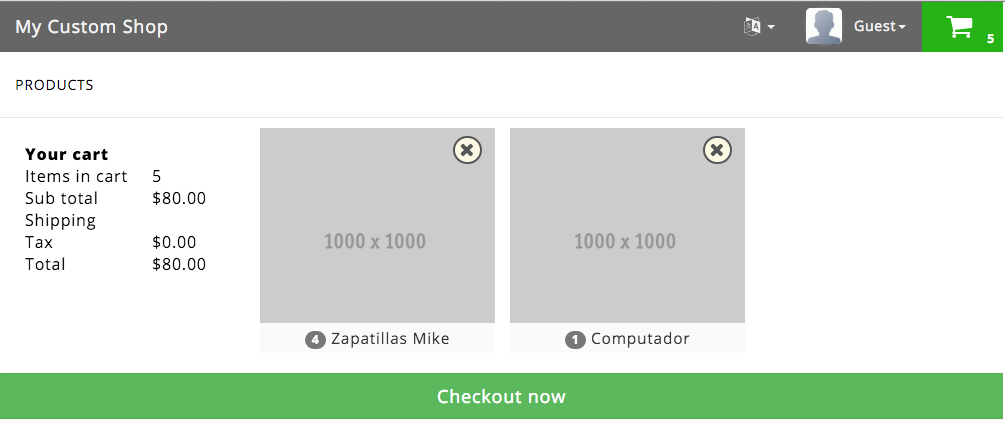
\includegraphics[width=0.8\textwidth]{figuras/solution/cart/view.png}
			\caption{Información global del carro. Tiene un resumen del costo total de los elementos seleccionados.}
			\label{figure:solution:cart:view}
		\end{figure}

		Cada uno de los diferentes elementos agregados al carro pueden ser eliminados simplemente presionando sobre la [x] que tiene asociada cada producto (\refFigura{figure:solution:cart:product}). Esto permite tener \textbf{control} sobre el contenido del carro. Es importante recordar como concepto general de diseño de interfaces, que es inevitable que las personas cometan errores, o incluso cambien de parecer durante algún procedimiento. Es necesario entonces permitir correcciones \cite{online_goodgui_org}. 

		\begin{figure}[H]
			\centering
			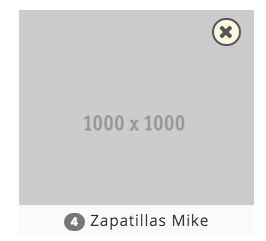
\includegraphics[width=0.5\textwidth]{figuras/solution/cart/producto.png}
			\caption{Vista básica de un producto seleccionado. La [x] permite eliminar ese producto del carro de compra.}
			\label{figure:solution:cart:product}
		\end{figure}

		El botón \checkoutNowLABEL que se ubica en la parte inferior de la vista \nameref{chapter:section:carro_compra:subsection:request} nos envía a la interfaz de \nameref{chapter:solucionimplementada:section:checkout}.

		De momento no es posible actualizar la cantidad de un determinado producto dentro del carro. En el caso particular del producto de la \refFigura{figure:solution:cart:product}, solo se pueden eliminar los 4 productos simultáneamente.




% caracteristicas actuales en profile
%!TEX root = ../../../memoria.tex
\section{Profile}

	La \uiSiglaAS de profile permite ver y editar información relacionada directamente con el usuario. Esta información está dividida en dos partes: actualización de contraseña y libreta de direcciones.

	\subsection{Actualizar contraseña}

		El formulario de actualización de contraseña permite al usuario cambiar tanto como desee la contraseña que tiene actualmente. Después de todo, el cambio periódico de una contraseña es una medida de seguridad básica \cite{zviran1999password}.
		%The periodic changing ofa password is a basic security measure  

		Como se puede observar en la \refFigura{figure:profile:form:form_update_password}, el formulario de actualización de contraseña cuenta con dos campos obligatorios para el proceso. El primero corresponde al campo de solicitud de contraseña actual (a modo de confirmación de que la persona que está actualizando la contraseña, sea el dueño de la cuenta) y el segundo campo, para ingresar la nueva contraseña. Al apretar el botón de confirmación esta se cambia.

		\begin{figure}[h!]
			\centering
			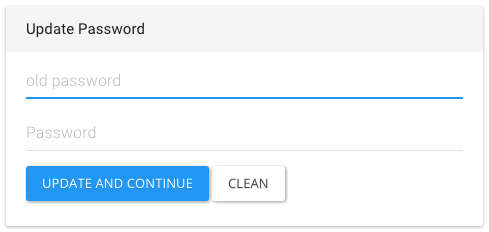
\includegraphics[width=0.5\textwidth]{figuras/profile/form_update_password.png}

			\caption{Formulario de actualización de contraseña.}
			\label{figure:profile:form:form_update_password}
		\end{figure}

		Existen diversas situaciones en donde el formulario notifica sobre errores que se cometen  al momento de llenar el formulario. Por ejemplo, al intentar enviar el formulario sin información ambos campos tienen errores y pueden observarse en la \refFigura{figure:profile:form:update_password:empty_form_send}.



		\begin{table}[h!]
		    \centering
			\begin{tabular}{ |l|c||l| }
				\hline Campo & Requerido & Restricción \\ \hline
				\multirow{1}{*}{\textit{Current Password}} 	&  \checkmark 					&  Debe ser la contraseña actual.\\ \hline
				\multirow{2}{*}{\textit{Password}} 			&  \multirow{2}{*}{\checkmark}	&  - Debe tener al menos 8 caracteres.\\
															&  								&  - Debe tener al menos un número o símbolo.\\ \hline
			\end{tabular}
		 	\caption{Resumen restricciones formulario edición de contraseña (\refFigura{figure:apendice:profile:form:update_password:empty_form_send}  y \refFigura{figure:apendice:profile:form:update_password:week_password}).}
		    \label{tab:profile:form:restrictions:update_password}
		\end{table}


		Tanto en la \refFigura{figure:apendice:profile:form:update_password:empty_form_send} y en la \refFigura{figure:apendice:profile:form:update_password:week_password} se puede observar que la nueva contraseña no cumple con estos requerimientos.
		Los requerimientos solicitados no responden a ninguna política de seguridad actual. Simplemente se eligieron esos requerimientos para evitar contraseñas aún más débiles que las que se pueden generar.


		Existe un último error, y corresponde simplemente cuando el usuario no logra identificarse correctamente, o lo que es equivalente, la contraseña actual ingresada no es correcta. En la \refFigura{figure:apendice:profile:form:update_password:incorrect_password} puede observarse el mensaje que el formulario entrega en este caso.


		% \subsubsection{Ordenes de compra}

		% 	El backend de las ordenes de compra aún no esta terminado, de momento solo esta el mensaje cuando no hay ninguna orden (\refFigura{figure:profile:orders_empty}).

		% 	\begin{figure}[h!]
		% 	\centering
		% 	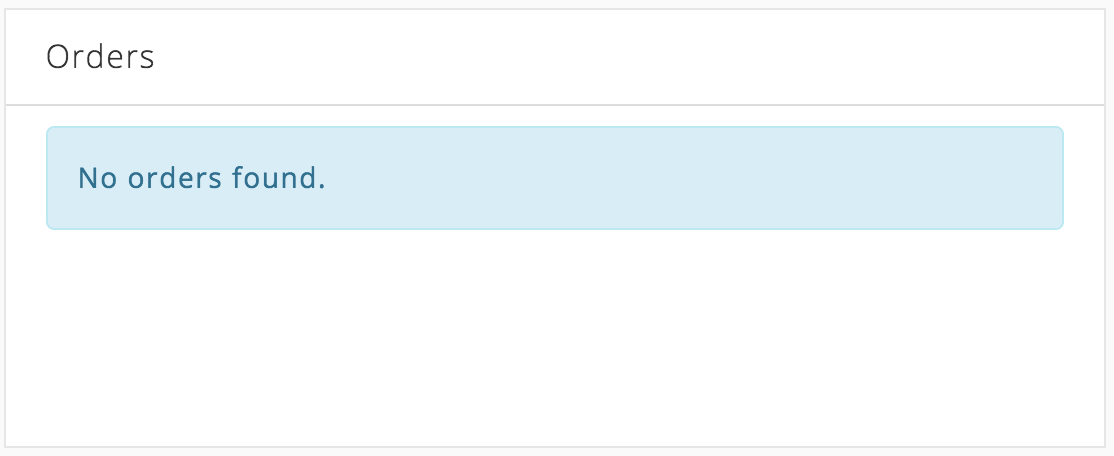
\includegraphics[width=0.5\textwidth]{figuras/profile/orders_empty.png}

		% 	\caption{Vista de ordenes cuando no hay ninguna.}
		% 	\label{figure:profile:orders_empty}
		% \end{figure}



	\subsection{Libreta de direcciones}\label{chapter:solucionimplementada:section:profile:subsection:book_address}

		Corresponde a todas las direcciones que el usuario ha agregado al sistema con el fin de utilizarlas para la recepción del o los productos y de las facturas. Cada uno de los parámetros del formulario para una dirección fue elegido a partir del formulario de direcciones que utiliza \amazonNAME (\refFigura{figure:apendice:address:example:amazon_address}).

		Como buena práctica, se debe utilizar la dirección de \ShippingCOM como dirección \defaultCPT para la dirección de facturación. Los clientes típicamente ordenan productos para la dirección del hogar. Así que por \defaultCPT, se debe utilizar la misma dirección para ambos casos\cite{online_official_smashingmagazine_fundamental_guidelines_checkout_design}.
		%8. Use Shipping Address As Billing Address By Default Link
		% Issue: Most customers order products to their home, so requiring both a billing and shipping address doesn’t make sense.
		% Customers typically order products to their home address. So, by default, you should use the same address for shipping and billing, unless you happen to record data differently for your store.
		Dejando la dirección de facturación por \defaultCPT como la de \ShippingCOM, el proceso de \checkoutCOM tendrá algunos campos menos, haciendo el proceso menos intimidante para los clientes. Los usuarios también disminuyen el riesgo de cometer un error al escribir sus direcciones solo una vez; ellos no se moverán a través del formulario de manera tan rápida y de existir errores, el usuario solo tendrá que resolverlos una vez \cite{online_official_smashingmagazine_fundamental_guidelines_checkout_design}.
		% By defaulting the billing address to the shipping address, your checkout process will have many fewer fields, making it less intimidating for customers. Users also reduce the risk of misspelling their address if they have to enter it only once; they won’t rush through the form as quickly, and if there are errors, the customer will have to fix them only once.

		Teniendo en consideración estos detalles, se desarrolla el formulario que se observa en la \refFigura{figure:address:form:add_new_address}.

		\begin{figure}[h!]
			\centering
			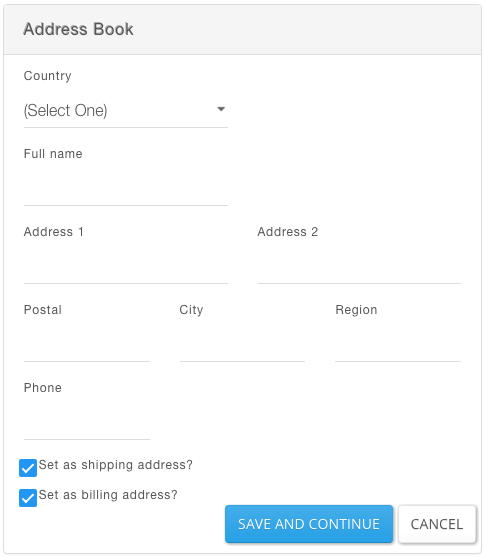
\includegraphics[width=1\textwidth]{figuras/address/form/add_new_address.png}
			\caption{Formulario para agregar una nueva dirección.}
			\label{figure:address:form:add_new_address}
		\end{figure}

		Este formulario cuenta con las restricciones descritas en la \reftabla{tab:profile:form:restrictions:address}, y por lo tanto muestra mensaje de error según corresponda.
		%TODO : Agregar figuras del formulario con diferentes tipos de errores en el apendice y referenciarlos acá

		\begin{table}[h!]
		    \centering
			\begin{tabular}{ |l|c||l| }
				\hline Campo & Requerido & Restricción \\ \hline
				\multirow{1}{*}{\textit{Country}} 			&  \checkmark 	&  Debe ser una de las alternativas.\\ \hline
				\multirow{1}{*}{\textit{Full Name}} 		&  \checkmark	& \\ \hline
				\multirow{1}{*}{\textit{Address 1}} 		&  \checkmark	& \\ \hline
				\multirow{1}{*}{\textit{Address 2}} 		&  				& \\ \hline
				\multirow{1}{*}{\textit{Postal}} 			&  \checkmark	& \\ \hline
				\multirow{1}{*}{\textit{City}} 				&  \checkmark	& \\ \hline
				\multirow{1}{*}{\textit{Region}} 			&  \checkmark	& Para ciertos países, existen alternativas definidas.\\ \hline
				\multirow{1}{*}{\textit{Phone}} 			&  \checkmark	& \\ \hline
				\multirow{1}{*}{\textit{Shipping address}} 	&  \checkmark	& Boolean. \\ \hline
				\multirow{1}{*}{\textit{billing address}} 	&  \checkmark	& Boolean. \\ \hline
				\multirow{1}{*}{\textit{comercial address}} &  \checkmark	& Boolean. \\ \hline
			\end{tabular}
		 	\caption{Resumen restricciones formulario para libreta de direcciones.}
		    \label{tab:profile:form:restrictions:address}
		\end{table}

		Notar que en la parte superior de la \refFigura{figure:address:form:add_new_address} está el botón que permite ingresar nuevas direcciones. Cada una de estas nuevas direcciones es agregada a la lista que aparece en la \refFigura{figure:address:form:list_address}, lugar en donde pueden ser editadas y eliminadas de acuerdo a las necesidades del cliente. En caso de editar alguna dirección, esta debe cumplir las mismas restricciones impuestas para el caso de la creación de una dirección (\reftabla{tab:profile:form:restrictions:address}).

		\begin{figure}[h!]
			\centering
			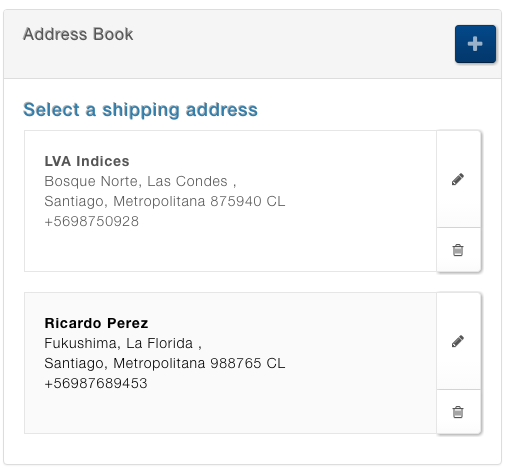
\includegraphics[width=1\textwidth]{figuras/address/form/list_address.png}
			\caption{Lista con todas las direcciones configuradas del usuario. Cada una de estas puede ser editada o eliminada con los botones que se encuentran en el costado derecho.}
			\label{figure:address:form:list_address}
		\end{figure}

		Es importante agregar que en la situación en que el usuario no tenga configurada ninguna dirección, aparecerá por \defaultCPT el formulario de creación. Esto se observa en la \refFigura{figure:address:form:add_first_address}.

		\begin{figure}[h!]
			\centering
			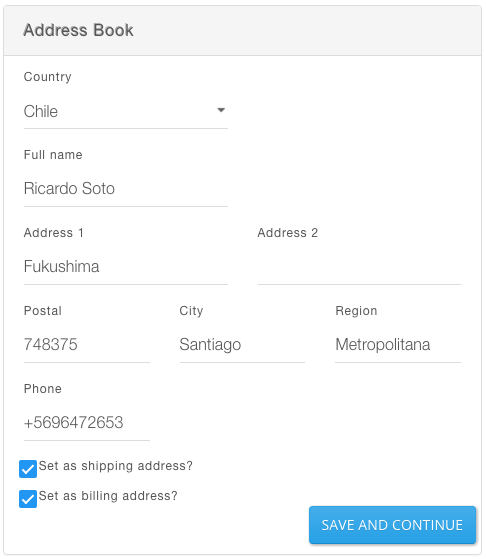
\includegraphics[width=1\textwidth]{figuras/address/form/add_first_address.png}
			\caption{Formulario para agregar una nueva dirección, aparece en caso de no existir configurada ninguna previa. Notar que no existe un botón para cancelar dado que en este contexto no tiene sentido.}
			\label{figure:address:form:add_first_address}
		\end{figure}






% caracteristicas actuales en dashboard
%!TEX root = ../../../memoria.tex
\section{\dashboardEF}
	Corresponde al administrador de características de la aplicación. Básicamente muestra todas las funcionalidades customizables que existen en la plataforma.
	%Cada package agregado el proyecto contiene el archivo \packageDescriptionFILE, el cual proporciona al \dashboardEF la información necesaria para agregar una o más componentes a la \uiSiglaAS con información descriptiva y con el link hacia la pantalla de configuración.
	La información que se muestra de cada componente corresponde a:

	\begin{itemize}
		\item Nombre de la componente a agregar.
		%\item Descripción breve de la componente.
		\item Un icono.
	\end{itemize} 

	En la \refFigura{figure:dashboard:main_menu} se observa el \dashboardEF 5 elementos configurables de la aplicación. 

	\begin{figure}[!h]
		\centering
		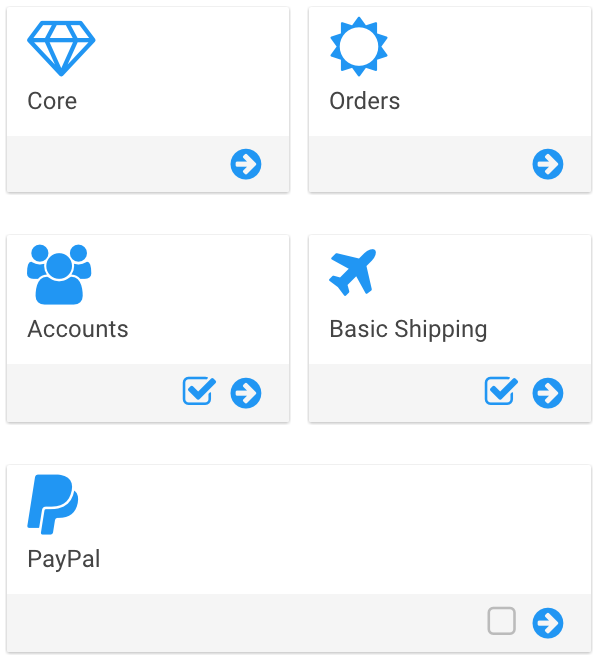
\includegraphics[width=0.6\textwidth]{figuras/dashboard/main_menu.png}
		\caption{\dashboardEF con elementos configurables de la aplicación.}
		\label{figure:dashboard:main_menu}
	\end{figure}

	Existen ciertos \packagesAS que tienen la opción de ser deshabilitados. Esta opción es especialmente útil para agregar o quitar ciertas funcionalidades al \websiteINT. A modo de ejemplo, en la \refFigura{figure:dashboard:paypal_disabled} se observa que el \packageAS de \paypalNAME está deshabilitado, en contraste con el \packageAS de \ShippingCOM. En el caso de que existieran más opciones de pago como \googleWalletNAME y \amazonPayments, se podrían ocultar los métodos sencillamente utilizando este método.

	\begin{figure}[!h]
		\centering
		
\includegraphics[width=0.4\textwidth]{figuras/dashboard/paypal_disabled.png}
		\caption{\dashboardEF con elementos configurables de la aplicación.}
		\label{figure:dashboard:paypal_disabled}
	\end{figure}

	% Dashboar Core
	%!TEX root = ../../../../memoria.tex
\subsection{\ecomFrameworkCoreEF}

Corresponde a la customización de los elementos relacionados directamente con la tienda. La información se ha jerarquizado en diferentes paneles de contenido plegable (conocidos como menú acordeón) los cuales se observan en la \refFigura{figure:dashboard:ecommerce:main_menu}.
%Displays collapsible content panels for presenting information in a limited amount of space.
\begin{figure}[H]
	\centering
	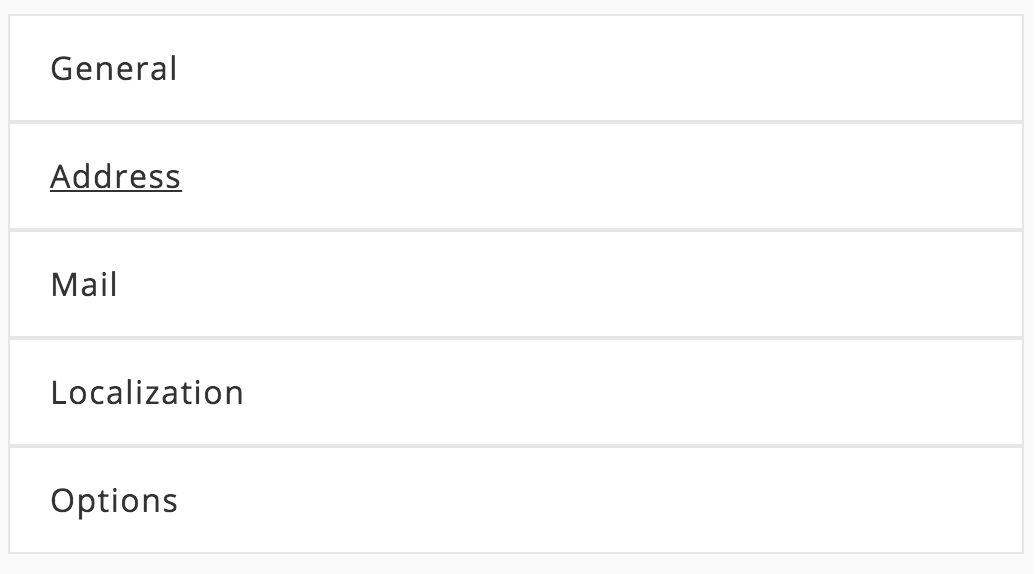
\includegraphics[width=0.6\textwidth]{figuras/dashboard/ecommerce/main_menu.png}
	\caption{Menú general de \ecomFrameworkCoreEF.}
	\label{figure:dashboard:ecommerce:main_menu}
\end{figure}

Cada uno de estos elementos tiene información configurable, además del \feedback habitual correspondiente a la información entregada de validación de cada campo, tiene una ventana emergente para indicar si la actualización del formulario fue o no exitosa.
La rázon de esta información extra es muy sencilla, si no existieran estos mensajes emergentes, estaría la ambigüedad de si el resultado fue exitoso o no dado que no hay ningún otro elemento gráfico con el cual se podría inferir el resultado. Por ejemplo, el formulario no se \'limpia\', el formulario no se cierra, no se agrega un nuevo elemento a una lista, etc.

\begin{figure}[H]
	\centering
	
\includegraphics[width=0.6\textwidth]{figuras/dashboard/ecommerce/success_message.png}
	\caption{Mensaje de confirmación de éxito en la actualización del formulario. Este mensaje se esconde después de un breve intervalo de tiempo.}
	\label{figure:dashboard:ecommerce:success_message}
\end{figure}

\begin{figure}[H]
	\centering
	
\includegraphics[width=0.8\textwidth]{figuras/dashboard/ecommerce/error_message.png}
	\caption{Mensaje para informar sobre un error en el proceso de actualización del formulario.}
	\label{figure:dashboard:ecommerce:error_message}
\end{figure}

En el caso de ser exitoso, aparece un mensaje el cual eventualmente desaparecerá de un breve intervalo de tiempo(\refFigura{figure:dashboard:ecommerce:success_message}). Los mensajes de error persisten en el tiempo. Por lo tanto se deben cerrar para que desaparezcan (\refFigura{figure:dashboard:ecommerce:error_message}).


\subsubsection*{Panel \generalPanel}

El panel general está formado por dos formularios; el primero solo contiene un campo y es un checkbox para permitir que un usuario \userGuestAccount pueda realizar un \checkoutCOM (\refFigura{figure:dashboard:ecommerce:general_menu:allow_checkout}).

\begin{figure}[H]
	\centering
	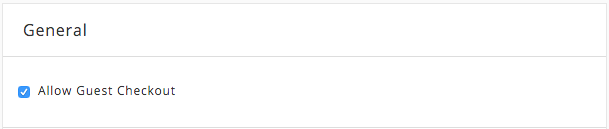
\includegraphics[width=0.6\textwidth]{figuras/dashboard/ecommerce/general_menu/allow_checkout.png}
	\caption{Formulario de información general de la tienda}
	\label{figure:dashboard:ecommerce:general_menu:allow_checkout}
\end{figure}

Este formulario tiene la particuladidad que se envía automáticamente al cambiar su estado.
El otro formulario está relacionado con la información más general de la empresa ( \refFigura{figure:dashboard:ecommerce:general_menu:menu})

\begin{figure}[H]
	\centering
	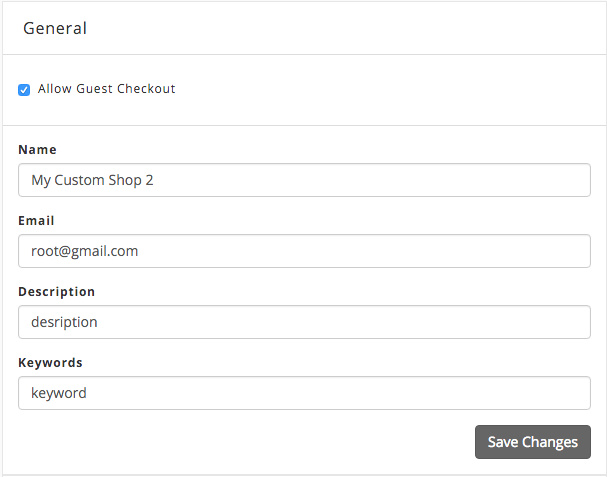
\includegraphics[width=0.6\textwidth]{figuras/dashboard/ecommerce/general_menu/menu.png}
	\caption{Formulario de información general de la tienda}
	\label{figure:dashboard:ecommerce:general_menu:menu}
\end{figure}

\begin{table}[H]
    \centering
	\begin{tabular}{ |l|c||l| }
		\hline Campo & Requerido & Restricción \\ \hline
		\multirow{1}{*}{\textit{Name}} 			&  {\checkmark} &  \\ \hline
		\multirow{1}{*}{\textit{Email}} 		&  				&  Debe ser un email válido.\\ \hline
		\multirow{1}{*}{\textit{Description}} 	&  				&  \\ \hline
		\multirow{1}{*}{\textit{Keywords}} 		&  				&  \\ \hline
		\hline
	\end{tabular}
 	\caption{Restrincciones formulario \generalPanel}
    \label{tab:dashboard:ecommerce:form:general}
\end{table}


Este formulario solo tienen un campo obligatorio, y corresponde a \textit{Name}. Al igual que otros formularios, dicho campo se destaca de color rojo, además de entregar un mensaje a modo de identificar el error (\refFigura{figure:apendice:dashboard:ecommerce:general_menu:updated_error}).



\subsubsection*{Panel \addressPanel}\label{capitulo:solucionImplementada:dashboard:subsubsection:addressPanel}

Este formulario se utiliza para agragar información física de la tienda, como algún teléfono de contacto.

\begin{figure}[H]
	\centering
	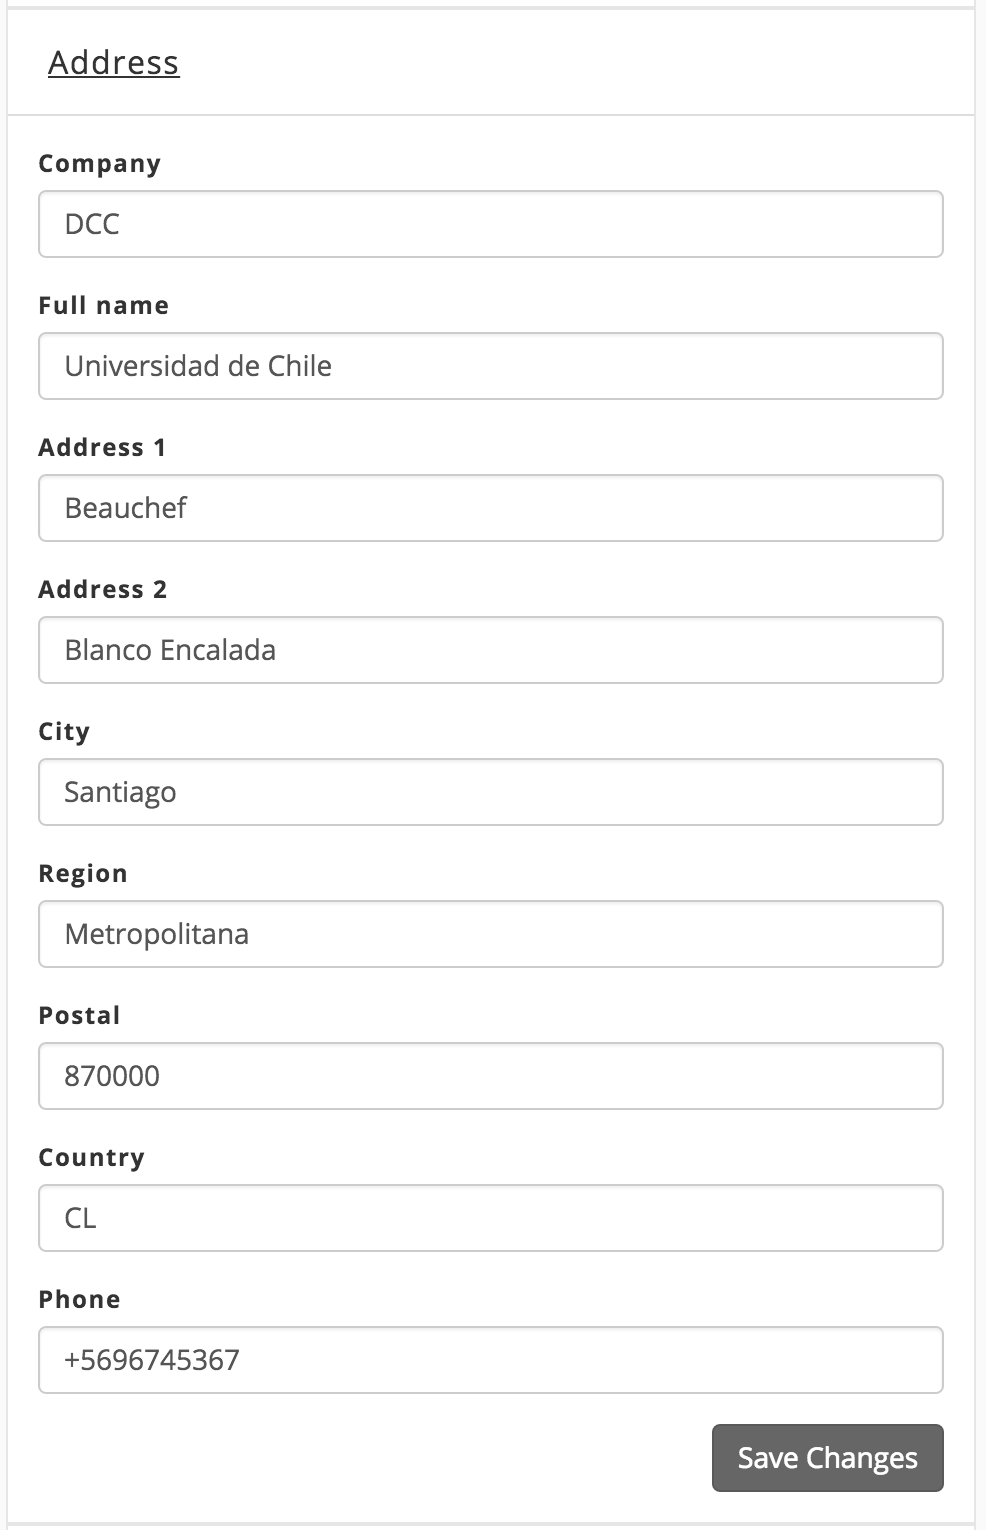
\includegraphics[width=0.5\textwidth]{figuras/dashboard/ecommerce/address/menu.png}
	\caption{Formulario de la dirección física de la tienda.}
	\label{figure:dashboard:ecommerce:address:menu}
\end{figure}

En relación a los campos del formulario, se tienen las siguientes restricciones (\reftabla{tab:dashboard:ecommerce:form:address}):

\begin{table}[H]
    \centering
	\begin{tabular}{ |l|c||l| }
		\hline Campo & Requerido & Restricción \\ \hline
		\multirow{1}{*}{\textit{Full name}} &  {\checkmark} &  \\ \hline
		\multirow{1}{*}{\textit{Address 1}} &  {\checkmark} &  \\ \hline
		\multirow{1}{*}{\textit{Address 2}} &   			&  \\ \hline
		\multirow{1}{*}{\textit{City}} 		&  {\checkmark} &  \\ \hline
		\multirow{1}{*}{\textit{Region}} 	&  {\checkmark} &  \\ \hline
		\multirow{1}{*}{\textit{Postal}} 	&  {\checkmark} &  \\ \hline
		\multirow{1}{*}{\textit{Country}}	&  {\checkmark} &  \\ \hline
		\multirow{1}{*}{\textit{Phone}} 	&  {\checkmark} &  \\ \hline
	\end{tabular}
 	\caption{Restrincciones formulario \addressPanel}
    \label{tab:dashboard:ecommerce:form:address}
\end{table}


\subsubsection*{Panel \mailPanel}

Corresponde a la información básica necesaria para configurar un servicio de \email. Agregar un \email no es requerido, pero si se configura el servicio deben agregarse tódos los campos(\reftabla{tab:dashboard:ecommerce:form:mail}).

\begin{figure}[H]
	\centering
	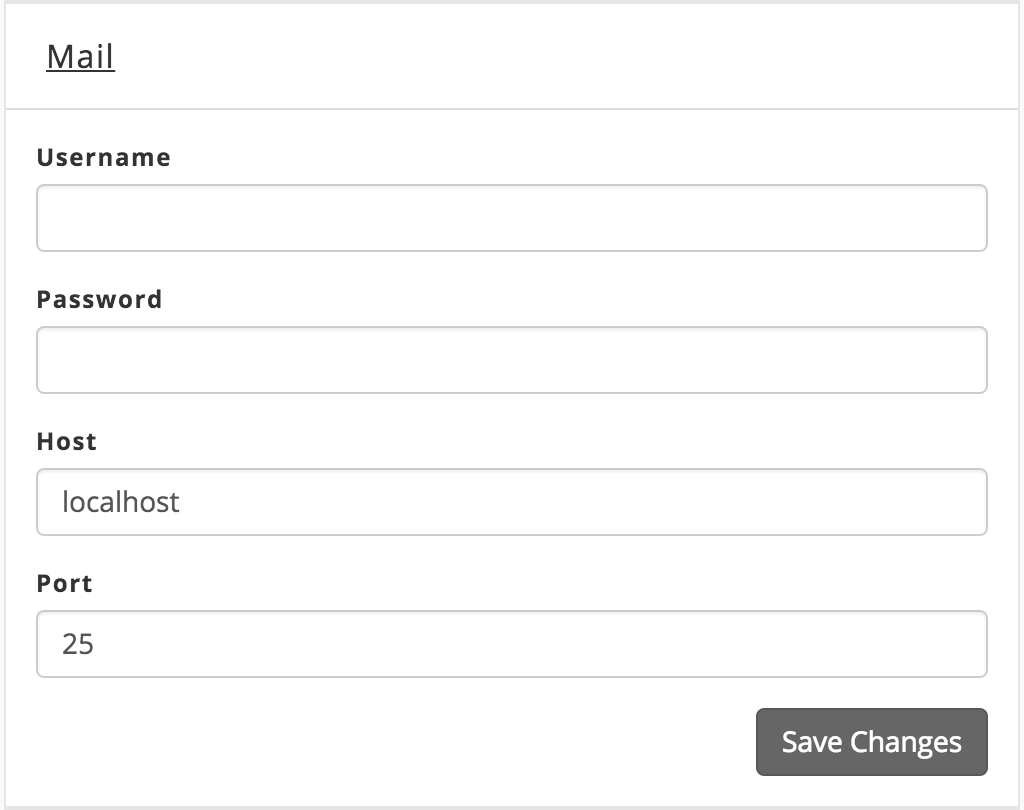
\includegraphics[width=0.6\textwidth]{figuras/dashboard/ecommerce/mail/menu.png}
	\caption{Formulario con la información de la configuración del Mail.}
	\label{figure:dashboard:ecommerce:mail:menu}
\end{figure}

\begin{table}[H]
    \centering
	\begin{tabular}{ |l|c||l| }
		\hline Campo & Requerido & Restricción \\ \hline
		\multirow{1}{*}{\textit{User Name}} &  {\checkmark} &  \\ \hline
		\multirow{1}{*}{\textit{Password}} 	&  {\checkmark} &  \\ \hline
		\multirow{1}{*}{\textit{Host}} 		&  {\checkmark} &  \\ \hline
		\multirow{1}{*}{\textit{Port}} 		&  {\checkmark} & Número mayor que 0 \\ \hline
		\hline
	\end{tabular}
 	\caption{Restrincciones formulario \mailPanel}
    \label{tab:dashboard:ecommerce:form:mail}
\end{table}


\subsubsection*{Panel \optionsPanel}

\begin{figure}[H]
	\centering
	\includegraphics[width=0.6\textwidth]{figuras/dashboard/ecommerce/options/menu.png}
	\caption{Formulario con información relacionada con los Analytics.}
	\label{figure:dashboard:ecommerce:options:menu}
\end{figure}

\begin{table}[H]
    \centering
	\begin{tabular}{ |l|c||l| }
		\hline Campo & Requerido & Restricción \\ \hline
		\multirow{1}{*}{\textit{Open Exchange}} 	&  {\checkmark} &  \\ \hline
		\multirow{1}{*}{\textit{Google Client}} 	&  {\checkmark} &  \\ \hline
		\multirow{1}{*}{\textit{Google Api}} 		&  {\checkmark} &  \\ \hline
		\hline
	\end{tabular}
 	\caption{Restrincciones formulario \optionsPanel}
    \label{tab:dashboard:ecommerce:form:options}
\end{table}

	% Dashboar Orders
	%!TEX root = ../../../../memoria.tex
\subsection{\ordersEF}

	Por definición, una orden corresponde a una solicitud confirmada, en esta caso particular, desde un cliente para comprar un \itemCOM o servicio bajo unos términos y condiciones específicas. Es importante mencionar que el flujo de compra no ha terminado cuando el cliente a realizado el pago. Es en este escenario en donde surge el concepto de \orderFulfillmentCOM.
	Esta sección permite al encargado administrar las ordenes generadas por los clientes para posteriormente gestionarlas, conteniendo por lo tanto, toda la información necesaria para llevar a cabo dicho proceso.
	Dada la complejidad de operaciones que puede alcanzar \orderFulfillmentCOM, en la aplicación, está sección se ha simplificado a lo más fundamental.

	Al selección las Ordenes desde el panel de \dashboardEF, lo primero que se vera es la lista de todas las Ordenes ingresadas por los clientes que se encuentran actualmente en el sistema. En la \refFigura{figure:dashboard:orders:grid} se ve la pantalla de Ordenes.


	\begin{figure}[H]
		\centering
		\includegraphics[width=0.6\textwidth]{figuras/dashboard/orders/grid.png}
		\caption{Vista general de todas las ordenes ingresadas por clientes.}
		\label{figure:dashboard:orders:grid}
	\end{figure}

	Cada una de estas ordenes estan disponibles para realiar acciones sobre ellas. Estas acciones radican principalmete en cambiar el estado actual de la orden. El detalle de la orden se ve en la \refFigura{figure:dashboard:orders:orderInfo}
%TODO agregar mas información sobre la orden.
	\begin{figure}[H]
		\centering
		\includegraphics[width=0.6\textwidth]{figuras/dashboard/orders/orderInfo.png}
		\caption{Detalle de orden ingresada por un cliente.}
		\label{figure:dashboard:orders:orderInfo}
	\end{figure}

	% Dashboar accounts
	%!TEX root = ../../../../memoria.tex
\subsection{\accountsEF}

	Permite agregar o quitar permisos a los usuarios. El sistema actualmente permite crear usuarios y modificar sus permisos permitiendo o eliminando las componentes relacionadas a sus permisos.

	\begin{figure}[H]
		\centering
		\includegraphics[width=0.6\textwidth]{figuras/dashboard/account/users.png}
		\caption{Interfaz con los usuarios del sistema.}
		\label{figure:dashboard:account:users}
	\end{figure}


	\begin{figure}[H]
		\centering
		\includegraphics[width=0.6\textwidth]{figuras/dashboard/account/permisos.png}
		\caption{Interfaz para administrar los permisos del sistema.}
		\label{figure:dashboard:account:permisos}
	\end{figure}

\begin{table}[H]
    \centering
	\begin{tabular}{ |l|c||l| }
		\hline Campo & Requerido & Restricción \\ \hline
		\multirow{1}{*}{\textit{Core}} 			&  \checkmark 	& Boolean \\ \hline
		\multirow{1}{*}{\textit{Dashboard}} 	&  \checkmark	& Boolean \\ \hline
		\multirow{1}{*}{\textit{Orders}} 		&  \checkmark	& Boolean \\ \hline
		\multirow{1}{*}{\textit{Add Product}} 	&  \checkmark	& Boolean \\ \hline
		\multirow{1}{*}{\textit{Accounts}} 		&  \checkmark	& Boolean \\ \hline
		\multirow{1}{*}{\textit{Profile}} 		&  \checkmark	& Boolean \\ \hline
		\multirow{1}{*}{\textit{Shipping}} 		&  \checkmark	& Boolean \\ \hline
	\end{tabular}
 	\caption{Resumen restrincciones formulario para los permisos.}
    \label{tab:dashboard:account:form:restrictions:account}
\end{table}

	% Dashboar shipping
	%!TEX root = ../../../../memoria.tex
\subsection{\shippingEF}\label{cap:solucionImplementada:section:dashboard:subsection:shipping}

\shippingEF es parte del proceso realmente grande y complejo perteneciente al \workflowCPT \orderFulfillmentCOM. 

Como primer paso, hay que agregar una dirección de origen, la cual es agreagada en \nameref{capitulo:solucionImplementada:dashboard:subsubsection:addressPanel}.

Segundo, se deben agregar \shippingZonesCOM los cuales tendran su correspondiente \shippingRatesCOM. Existen servicios que permiten calcular en tiempo real el \shippingRatesCOM, evitando así que la tienda asuma un costo extra por un error en la estimación de la tarifa de envío. El sitio además debería ser capaz de determinar, si la dirección de destino se encuentra dentro de alguna de las \shippingZonesCOM definidas.

% TODO falta agregar descripcion del proceso
%https://docs.shopify.com/manual/shipping/initial-shipping-setup#add-a-shipping-zone

Por temás de tiempo, se decidío simplificar la solución, permitiendo agregar diferentes opciones de \shippingEF que eventualmente representarían diferentes criterios de envío.

%TODO Agregar mas informaciñon 

\begin{figure}[H]
	\centering
	\includegraphics[width=0.6\textwidth]{figuras/dashboard/shipping/shipping_options.png}
	\caption{Tabla con todas las opciones de \shippingEF disponibles.}
	\label{figure:dashboard:shipping:shipping_options}
\end{figure}

\begin{table}[H]
    \centering
	\begin{tabular}{ |l|c||l| }
		\hline Campo & Requerido & Restricción \\ \hline
		\multirow{1}{*}{\textit{Method Name}} 	&  \checkmark 	& \\ \hline
		\multirow{1}{*}{\textit{Public Label}} 	&  \checkmark	& \\ \hline
		\multirow{1}{*}{\textit{Group}} 		&  \checkmark	& \\ \hline
		\multirow{1}{*}{\textit{Cost}} 			&  				& \\ \hline
		\multirow{1}{*}{\textit{Handling}} 		&  				& \\ \hline
		\multirow{1}{*}{\textit{Rate}} 			&  \checkmark	& Número mayor que 0. \\ \hline
		\multirow{1}{*}{\textit{Enabled}} 		&  \checkmark	& Boolean \\ \hline
		\hline
	\end{tabular}
 	\caption{Resumen restrincciones formulario para \shippingEF.}
    \label{tab:dashboard:shipping:form:restrictions:shipping}
\end{table}

\begin{figure}[H]
	\centering
	\includegraphics[width=0.6\textwidth]{figuras/dashboard/shipping/form_shipping_add.png}
	\caption{Formulario para la creación de \shippingEF.}
	\label{figure:dashboard:shipping:form_shipping_add}
\end{figure}



\begin{figure}[H]
	\centering
	\includegraphics[width=0.6\textwidth]{figuras/dashboard/shipping/form_shipping_update.png}
	\caption{Formulario de actualización un \shippingEF.}
	\label{figure:dashboard:shipping:form_shipping_update}
\end{figure}


\subsubsection{Tarifas de \shippingEF y carros abadonados}

Aunque no es un tema que involucre a la finalidad de esta memoeria, es importante mencionar la importancia que tiene el factor \shippingEF dentro del abandono del carro de compra.
El desafio real que aparece cuando se desea abordar la estrategía de \shippingEF, es determinar la solución que impacte lo mínimo posible los margenes, pero que aún asi siga siendo atractivo para el cliente.
Y esto es algo en lo que se va querer estar en lo correcto. Estudios demuestran que el costo de \shippingEF es la principal razón del abandano de carros de compra (\refFigura{figure:dashboard:shipping:key_factor_shopping_cart_abandonment})\cite{online_forrester_consulting_smarter_stratefie_free_shipping}.

\begin{figure}[H]
	\centering
	\includegraphics[width=1\textwidth]{figuras/dashboard/shipping/key_factor_shopping_cart_abandonment.png}
	\caption{\shippingEF es un factor clave hacia el abandono de carros de compra \cite{online_forrester_consulting_smarter_stratefie_free_shipping}.}
	\label{figure:dashboard:shipping:key_factor_shopping_cart_abandonment}
\end{figure}

	% Dashboar payment
	%!TEX root = ../../../../memoria.tex
\subsection{\paymentsCOM}\label{cap:solucionImplementada:section:dashboard:subsection:payment}
	En establecimientos tradicionales \brickandmortar , un cliente ve un producto, lo examina, y entonces paga utlizando dinero, cheques, o tarjetas de crédito.
	% In traditional brick-and-mortar establishments, a customer sees a product, examines
	% it, and then pays for it by cash, check, or credit card (see Figure 6-1).

	En el mundo \ecommerceCOM, en la mayoría de los casos un cliente no ve fiscamente el producto al momento de realizar la transacción, y el método de pago es realizado electrónicamente. Por lo tanto, temas de confianza y aceptación juegan un rol más importante en el mundo \ecommerceCOM, que en el mundo de negocios tradicionales en lo que a sistemas de pago se refiere \cite{bidgoli2002electronic}.
	% In the e-commerce world, in most cases the customer does not physically see
	% the actual product at the time of transaction, and the method of payment is performed
	% electronically. Therefore, issues of trust and acceptance play a more important
	% role in the e-commerce world than in traditional businesses as far as payment
	% systems are concerned.

	Los sistemas de pago electrónico (\epsSiglasCOM, siglas en ingles) utilizan \hardwarePC y \softwarePC que permiten a los clientes pagar por productos y servicios en linea. Aunque estos sistemas podrían ser considerados inmaduros por los más críticos, no puede negarse el constante avance que viven periodicamente. El principal objetivo de un \epsSiglasCOM son incrementar eficiencia, mejorar seguridad, y lograr una mayor comodidad y facilidad de uso para los clientes \cite{bidgoli2002electronic}.
	% EPSs utilize integrated hardware and software systems that enable a customer
	% to pay for the goods and services online. Although these systems are in their infancy,
	% some significant progress has been made. The main objectives of EPS are
	% to increase efficiency, improve security, and enhance customer convenience and
	% ease of use. As shown throughout this chapter, there are several methods and
	% instruments that can be used to enable EPS implementation (see Figure
	% 6-2.)

	%Provide a Number of Payment Methods
	% 	It sounds obvious, but there are websites that offer only one payment method. However, data highlighted in an infographic from Milo shows that 56% of respondents expect a variety of payment options on the checkout page.
	Es importante agregar varios metodhos de \paymentsCOM. Puede sonar obvio, pero existen métodos que aún ofrecen solo una manera de realizar un pago. Un estudio demuestra que el 56\% de usuarios experan una variedad de opciones de \paymentsCOM en la página de \checkoutCOM \cite{online_kissmetrics_easy_payment_process}.

	% While it’s not necessary – nor practical for that matter – to offer every conceivable payment method available, you’ll want to take a look at your target audience to see which payment methods they use.
	Aunque en la práctica es innecesario e inpracticable, ofrecer todos los métodos de pagos existentes, se deseará observar el publico objetivo para determinar cuales son los métodos que ellos utilizan. Entonces se agregaran aquellos para capturar a la mayoria de los visitantes al \websiteINT \cite{online_kissmetrics_easy_payment_process}.

	En el contexto de esta memoria, solo se implementará a \paypalNAME como servicio de pago.
	
	\subsubsection{\paypalNAME}

		\paypalNAME es un servicio global que mueve los montos de pago desde una tarjeta de crédito hacia el vendedor sin compartir la información financiera. \paypalNAME ofrece una variadad de productos y soluciones para aceptar pagos. De estos uno ha sido elegído para permitir el flujo completo de compra, pero siempre considerando la opción de agregas nuevos métodos en un futuro.

		% TODO: ver si alcanzo agregar el otro método
		%De estos, se han elegido dos los cuales han sido considerados adecuados para los requerimientos.

		%PayPal is a global service that moves the payment amount from your credit card to the merchant without sharing your financial information. %PayPal offers a variety of products and solutions for accepting payments. You can choose the solution that is best for your requirements, whether your goal is to get up and running as quickly as possible or to develop a fully customized payment experience.

		\subsection*{\PPPaymentProNAME}
			\PPPaymentProNAME es una solución customizable que permite a los vendedores mantener a los compradores dentro de su \websiteINT durante el proceso completo de \paymentsCOM y \checkoutCOM. Los vendedores pueden mantener sus propios sitios de \checkoutCOM personalizados y enviar transacciones a \paypalNAME, o es posible también tener un \hostCPT de \paypalNAME que tenga páginas de \checkoutCOM e incluso manejar la seguridad para las ventas y autorización. \PPPaymentProNAME puede aceptar pagos de \paypalNAME y  \paypalCreditNAME, al igual que con tarjetas de crédito de pago \cite{online_paypal_developer_acceptpayments}.
			% PayPal Payments Pro is a customizable solution that enables merchants to keep buyers on their website during the entire checkout and payment process. Merchants can host their own customized checkout pages and send transactions to PayPal, or they can have PayPal host the checkout pages and also manage security for sales and authorizations. PayPal Payments Pro can accept Paypal and PayPal credit payments, as well as credit and debit card payments. PayPal Payments Pro also includes an optimized mobile checkout experience. For details, see PayPal Payments Pro.

			Para el uso de este servicio, es necesaria la creación de una \paypalNAME \appINT. Toda la información necesaria se encuentra en la documentación para los desarrollodores \cite{online_paypal_developer_apps_credentials}, pero en resumen, lo relevante acá para lograr una configuración adecuada son 3 elementos:

				\begin{itemize}
					\item Existen dos ambientes de trabajo: \sandboxEnvPL y \liveEnvPL.
					\item \clientIDPayPal.
					\item \secretPayPal.
				\end{itemize}

			Tanto el \clientIDPayPal como el \secretPayPal dependen del ambiente en el cual me encuentro.

			Desde el \dashboardEF es posible acceder al menú configurable de \paypalNAME el cual permite agregar esta información (ver \refFigura{figure:payment:paypal:payflow_pro:form}).

			\begin{figure}[H]
				\centering
				\includegraphics[width=0.6\textwidth]{figuras/payment/paypal/form_address.png}
				\caption{Formulario para agregar la configuración necesaria para el uso de \paypalNAME \paypalPayFlowNAME.}
				\label{figure:payment:paypal:payflow_pro:form}
			\end{figure}

			El formulario de \paypalNAME se somete a las restricciones visibles en la \refTabla{tab:payment:paypal:payflow_pro:form}.

			\begin{table}[H]
			    \centering
				\begin{tabular}{ |l|c||l| }
					\hline Campo & Requerido & Restricción \\ \hline
					\multirow{1}{*}{\textit{Payflow enabled}} 	&  \checkmark 	& Boolean\\ \hline
					\multirow{1}{*}{\textit{Client ID}} 		&  				& \\ \hline
					\multirow{1}{*}{\textit{Secret}} 			&  				& \\ \hline
					\multirow{1}{*}{\textit{PayFlow Mode}} 		&  \checkmark	& Boolean \\ \hline
					\hline
				\end{tabular}
			 	\caption{Formulario para agregar la configuración necesaria para el uso de \paypalPayFlowNAME.}
			    \label{tab:payment:paypal:payflow_pro:form}
			\end{table}
			


% caracteristicas actuales en checkout
%!TEX root = ../../../memoria.tex
\section{\checkoutEF}\label{chapter:solucionimplementada:section:checkout}

	Una de las peores violaciones de usabilidad para un \websiteINT \ecommerceCOM corresponde a un proceso de \checkoutEF que no sea lineal. \websiteINT que no tengan un proceso de \checkoutEF lineal dejan a muchos de los usuarios confusos e intimidados. Al momento de realizar este estudio, tanto \walmartNAME como \zapposNAME tenian un proceso \checkoutEF no lieal \cite{online_official_smashingmagazine_fundamental_guidelines_checkout_design}.
	% One of the worst usability violations that we discovered in our testing was non-linear checkout processes. Websites with a non-linear checkout process left several of our test subjects confused and intimidated. At the time of testing, both Walmart and Zappos had a non-linear checkout process.

	% The typical way to “accidentally” end up with a non-linear checkout process is to create steps within steps. This happens, for example, when the customer has to set a “Preferred shipping address” (Walmart’s violation) or “Create an account” (Zappos’ violation) on a separate page, and is then redirected to a previous checkout step upon completion.
	% Below, you can see Walmart’s checkout flow in thumbnails (click image for larger view). Notice that it’s non-linear because the “Preferred shipping address” sub-step directs the user to a previous step:

	Afortunadamente, hacer el proceso completamente lineal no es dificil. En el caso de necesitar por ejemplo, un sub-paso tal como \textit{creación de una cuenta}, esta nunca debe redirigir a un paso previo en el proceso de \checkoutEF, en lugar de eso, debe dirigir al cliente al siguiente paso del proceso de \checkoutEF\cite{online_official_smashingmagazine_fundamental_guidelines_checkout_design}. 
	%Luckily, making the process completely linear is easy. In this case, a sub-step such as “Account creation” should never redirect to a previous step in the checkout process, but instead direct the customer to the next step in the checkout process.

	Esto es crítico por que el modelo mental de la mayoria de los compradores dicta que el proceso de \checkoutEF debería ser lineal. Al ver la misma página dos veces, la mayoria de los clientes concluye que el sitio tienen un error, porque esto ocurre cuando hay errores de validación. \cite{online_official_smashingmagazine_fundamental_guidelines_checkout_design}. 
	%This is critical because the mental model of most customers dictates that a checkout process should be linear. Upon seeing the same page twice, most customers would conclude that the website has an error, because this is what happens with validation errors.
	%As one test subject said, “This looks suspiciously like the page I was on before. Is there something I didn’t do correctly?”

	Para este \frameworkPC se ha implementado un proceso de \checkoutEF lineal el cual tiene los pasos que se aprecian en la \refFigura{figure:checkout:steps}.

	% \begin{figure}[H]
	% 	\centering
	% 	\includegraphics[width=0.7\textwidth]{figuras/shipping/global_status.png}
	% 	\caption{Estado actual del \workflowCPT del \shippingEF. En este caso se encuentra en la selección de la dirección.}
	% 	\label{figure:checkout:global_status}
	% \end{figure}

	\begin{figure}[!h]
		\centering
		\includegraphics[width=0.8\textwidth]{figuras/shipping/steps.png}
		\caption{Detalle de todos los pasos del \workflowCPT \shippingEF.}
		\label{figure:checkout:steps}
	\end{figure}

	Otro detalle importante a considerar es que mientras sea posible, hay que limitar el proceso de \checkoutEF a una sola página. En el caso de separar el proceso en algunas páginas, se debe incluir una barra de proceso para mostrar cuanto falta para terminar \cite{online_official_imediaconnection_best_practices_shopping_cart}.
	% Try to keep it to one page
	% If at all possible, limit the checkout process to a single page. If you must spread it out across a few pages, include a progress bar to show people how far they have left to go.
	% Read more at http://www.imediaconnection.com/content/36794.asp#6qlTEqOcCeTePmFQ.99

	Afortunadamente, ambas restricciones son una manera para lograr la otra. Por lo tanto se desarrollo el proceso incluyendo a ambas. Esto se observa en la \refFigura{figure:checkout:global_status}.

	\begin{figure}[H]
		\centering
		\includegraphics[width=0.7\textwidth]{figuras/shipping/global_status.png}
		\caption{Estado actual del \workflowCPT del \shippingEF. En este caso se encuentra en la selección de la dirección.}
		\label{figure:checkout:global_status}
	\end{figure}

	Cada uno de los pasos que aparecen en la \refFigura{figure:checkout:steps} son descritos a continuación.

	% Paso Cuenta de usuario
	%!TEX root = ../../../../memoria.tex
\subsection{Cuenta de usuario}\label{chapter:solucionimplementada:section:account}

	Nada irrita más a un cliente que ser forzado a crear una cuenta para lograr comprar algo \online. Despues de todo, comprar \online se supone debería ser sencillo. Es cierto que la creación de una cuenta hará que las comprar en el futuro sean mas sencillas, pero no aporta nada para la situación en cuestión \cite{online_official_imediaconnection_best_practices_shopping_cart}.
	% Don't require registration to complete checkout
	% Nothing irks a customer more than being forced to create an account in order to buy something online. After all, online shopping is supposed to be easy. Sure, having an account will make future purchases easier, but it does nothing for the situation at hand. Instead, give shoppers the option of creating an account once the transaction is complete.

	Es cierto que este \frameworkPC requiere la creación de una cuenta para lograr la compra de productos, sin embargo no es necesario confirmarla para poder comprar. Es cierto que esta no es la situación ideal, pero esta situación tampoco es del todo mala, dado la simplicidad en la \nameref{chapter:solucionimplementada:accounts:subsection:create} (\ref{chapter:solucionimplementada:accounts:subsection:create}). 

	% Paso selección shipping & billing address
	%!TEX root = ../../../../memoria.tex
\subsection{Detalles de dirección}\label{chapter:solucionimplementada:section:address}

	Esta sección funciona exactamente igual \nameref{chapter:solucionimplementada:section:profile:subsection:book_address} ( \ref{chapter:solucionimplementada:section:profile:subsection:book_address}). En otras palabras, aparte de seleccionar una direacción permite:

	\begin{itemize}
		\item Ver todas las direcciones configuradas en el sistema.
		\item Editar y/o eliminar las direcciones disponibles del sistema.
		\item Configurar una nueva dirección.
		\item En caso de no tener ninguna dirección configurada, muestra el fomulario de creación.
	\end{itemize}

	Como se indica en otras partes, es altamente deseable limitar el proceso de \checkoutCOM a una sola página \cite{online_official_imediaconnection_best_practices_shopping_cart}. Estas funcionalidades están alineadas con este principio. En caso de necesitar hacer alguna gestión en las direcciones, no sea necesario cambiar de página.
	Como ejemplo, en la \refFigura{figure:checkout:form_address_default} se observa el formluario de creación de una dirección dado que no existe ninguna configurada previamente.

	\begin{figure}[H]
		\centering
		\includegraphics[width=0.6\textwidth]{figuras/shipping/form_address.png}
		\caption{Despliegue automático del formulario de direcciones cuando no se tienen ninguna dirección agregada.}
		\label{figure:checkout:form_address_default}
	\end{figure}

	% Paso opciones de envío
	%!TEX root = ../../../../memoria.tex
\section{Opciones de \ShippingCOM}\label{chapter:solucionimplementada:section:shipping_options}

	En este paso es posible seleccionar alguno de los métodos disponibles de \ShippingCOM por el sitio de ventas (\refFigura{figure:shipping:checkout:select_option}). Como describió en la sección 

	\begin{figure}[!h]
		\centering
		\includegraphics[width=0.8\textwidth]{figuras/shipping/steps.png}
		\caption{Detalle de todos los pasos del \workflowCPT \shippingEF.}
		\label{figure:shipping:checkout:select_option}
	\end{figure}

	% Paso resumen de la compra
	%!TEX root = ../../../../memoria.tex
\subsection{Resumen de la compra}\label{chapter:solucionimplementada:checkout:review}

	Esta sección muestra un resumen de la compra que se esta realizando (ver \refFigura{figure:review:checkout:summary}). Esta información es parte del detalle completo que debe mostrar esta sección para dejar claro al cliente que es exactamente lo que esta comprando. Esto debe ser mejorado como trabajo futuro.

	\begin{figure}[!h]
		\centering
		\includegraphics[width=0.8\textwidth]{figuras/shipping/steps.png}
		\caption{Detalle de la compra dentro del proceso de \checkoutEF.}
		\label{figure:review:checkout:summary}
	\end{figure}

	% Paso add paymant to complete order
	%!TEX root = ../../../../memoria.tex
\subsection{\paymentsCOM}\label{chapter:solucionimplementada:section:payment}
	
	Como se mencionó en la sección \ref{cap:solucionImplementada:section:dashboard:subsection:payment} \nameref{cap:solucionImplementada:section:dashboard:subsection:payment}, es relevante considerar varios métodos de pagos, sin embargo en el contexto de esta memoria solo se ha integrado a \PPPaymentProNAME.


	\subsubsection{\PPPaymentProNAME}
		Anteriormente se había indicado que este método permite mantener a los clientes dentro del \websiteINT durante el proceso completo de \paymentsCOM y \checkoutCOM. Básicamente se ha implementado la aceptación de pago de tarjetas de crédito a través de un formulario dentro del \websiteINT. La información necesaria para la transacción se ve en \refCodigo{source:javascript:checkout:payment:paypal_accept_payments}.

		% JSON con la información necesaria para aceptar el pago con tarjetas de crédito
		%!TEX root = ../../../../memoria.tex

\medskip
\begin{lstlisting}[caption= Estructura de un \itemcollection, label=source:javascript:checkout:payment:paypal_accept_payments]
{	
	"intent": "sale",
	"payer":{
		"payment_method": "credit_card",
		"funding_instruments": [
			{
				"credit_card": {
					"number": "5500005555555559",
					"type": "mastercard",
					"expire_month": 12,
					"expire_year": 2018,
					"cvv2": 111,
					"first_name": "Betsy",
					"last_name": "Buyer"
				}
			}
		]
	},
	"transactions": [
		{
			"amount": {
				"total": "7.47",
				"currency": "USD"
			},
			"description": "This is the payment transaction description."
		}
	]
}
\end{lstlisting}

		De acá se desprende la información de la tarjeta:

		\begin{itemize}
			\item Número.
			\item Tipo de Tarjeta.
			\item Mes en que expira la tarjeta.
			\item Año en que expira la tarjeta.
			\item \cvvTWOCOM.
			\item Nombre.
			\item Apellido.
		\end{itemize} 

		Toda esta información debe ser entregada por el cliente, con el fin de gestionar el pago. Sin embargo, se sabe que el tipo de tajeta puede ser determinado a partir de los 6 primeros dígitos del número de tarjeta \cite{online_investopedia_meaning_IIN}. 

		Los campos de expiración de tarjeta de crédito pueden ser confusos para decifrar si no son escritos exactamente como están en las tarjetas de crédito. Algunos \websitesINT usan nombres de meses, mientras otros emplean una combinación de \nombreNumeroCPT, mientras y usan solo números. La manera correcta de dar los campos de formato es simplemente poner los campos de la misma manera en que aparecen en la tarjeta de crédito (solamente números). Esto minimiza la confusión y mala interpretación porque el usuario puede fácilmente verificar  los campos contra los de la tarjeta de crédito \cite{online_official_smashingmagazine_fundamental_guidelines_checkout_design}.

		Finalmente, se desarrolla el formulario de la \refFigura{figure:checkout:payment:paypal_payflow:form}, para que el cliente pueda efectuar el pago del producto y/o servicio.

		\begin{figure}[H]
			\centering
			\includegraphics[width=0.6\textwidth]{figuras/payment/credit_card_form.png}
			\caption{Formulario de la tarjeta de crédito para realizar el pago utilizando \PPPaymentProNAME.}
			\label{figure:checkout:payment:paypal_payflow:form}
		\end{figure}

		%TODO: agregar referencia a la interfaz de orde de compra.
		Una vez finalizado este proceso, se creará una orden de compra, la cual podría ser consultado en la interfaz de ordenes.

% caracteristicas actuales en orders
%!TEX root = ../../../memoria.tex
\section{\ordersEF}\label{chapter:solucionimplementada:section:orders}
%  FIXME : Nueva información agregada despues de revision de mi papa
Muestra información relevante relacionada con cada una de las compras realizadas en el sitio por el cliente autenticado (ver \refFigura{figure:orders:client:list_orders}). Los detalles de esta interfaz fueron inspirados en la página de \ordersEF del \websiteINT \dealextremeNAME (ver \refFigura{figure:apendice:orders:example:dx_list_orders}).  


\begin{figure}[H]
	\centering
	\includegraphics[width=0.1\textwidth]{figuras/orders/client/list_orders.jpg}
	\caption{Lista de las \ordersEF que tiene un cliente.}
	\label{figure:orders:client:list_orders}
\end{figure}

Es importante recordar que las \ordersEF desplegadas corresponden a las del usuario autenticado.

% caracteristicas actuales en seguridad
%!TEX root = ../../../memoria.tex

\section{Seguridad en un sitio \ecommerceCOM}\label{cap:seguridad}


	Seguridad en una aplicación \webINT es sobre todo entender seguridad de los dominios (\securityDomainCPT) y entender la superficie de ataque (\attackSurfaceCPT) entre esos dominios. En una aplicación de \meteorNAME, las cosas son muy simples:
	%Securing a web application is all about understanding security domains and understanding the attack surface between these domains. In a Meteor app, things are pretty simple:

	\begin{itemize}
			\item
				El código que se ejecuta en el servidor es confiable.
			\item
				Todo lo demás: código que se ejecuta en el cliente, la información enviada a través métodos y publicación de argumentos, etc; no puede ser confiable.
	\end{itemize}
	%Code that runs on the server can be trusted.
	%Everything else: code that runs on the client, data sent through Method and publication arguments, etc, can’t be trusted.
	En la práctica, esto significa que la mayoría de la seguridad y las validaciones se encuentran en la interacción entre estos dominios. En términos simples:
	%In practice, this means that you should do most of your security and validation on the boundary between these two domains. In simple terms:
	\begin{itemize}
			\item
				Validar y revisar todos los \inputCPT que provienen desde el cliente.
			\item
				No liberar ninguna información secreta al cliente \cite{online_meteor_security}.
	\end{itemize}
	%Validate and check all inputs that come from the client.
	%Don’t leak any secret information to the client.



	La seguridad en \internetINT se ha tornado un problema constante y creciente al mismo tiempo que nuevas tecnologías basadas en \internetINT y aplicaciones son desarrolladas.
	%Internet security has become a consistent and growing problem as new Internet-based technologies and applications are developed. The number of security violation related incidents continues to increase [6]. A reported incident can be as simple as a single computer being compromised or as severe as a complete network compromise involving hundreds of client computers. All Internet content you read, send, and receive carries a risk. The amount of security risks increases at the same time that dependence on information technology grows. This demands the need for a comprehensive security program and makes the job of those persons tasked with network security even harder.



\section{Seguridad en \eframeworkAF}

%Note: This entire API and all rule methods are available only in server code. As a security best practice, you should not define your security rules in client code or in server code that is sent to clients. Meteor allow/deny functions are documented as server-only functions, although they are currently available in client code, too.


\subsection{Autorización}

%api.use("alanning:roles@1.2.13");
% https://atmospherejs.com/alanning/roles
Se integra la asignación de permisos a los usuarios, para posteriormente verificar si cuenta o no con accesos a ciertos métodos de \meteorNAME o publicar información.
%This package lets you attach permissions to a user which you can then check against later when deciding whether to grant access to Meteor methods or publish data. The core concept is very simple, essentially you are attaching strings to a user object and then checking for the existance of those strings later. In some sense, it is very similar to tags on blog posts. This package provides helper methods to make the process of adding, removing, and verifying those permissions easier.

La aplicación permite la flexibilidad de asignar permisos de la manera que parezca más útil. Se pueden utilizar roles tradicionales, como \textit{admin} o \textit{webmaster}, o incluso asignar permisos con una mayor granularidad tales como \verMensajesSecretosCPT, \vistaUsuariosCPT, \lecturaPlanillasCPT, etc. En general, una mayor granularidad es mejor, porque permite el manejo de aquellos casos particulares que existen en la \vidaRealCPT de forma sencilla, sin la necesidad de incluir una gran cantidad de \textit{roles}.

% Permissions vs roles (or What's in a name...)
% Although the name of this package is 'roles', you can define your permissions however you like. They are essentially just tags that you assign on a user and which you can check for later.

% You can have traditional roles like, "admin" or "webmaster", or you can assign more granular permissions such as, "view-secrets", "users.view", or "users.manage". Often times more granular is actually better because you are able to handle all those pesky edge cases that come up in real-life usage without creating a ton of higher-level 'roles'. To the roles package, it's all strings.


En ocasiones es útil permitir la asignación de conjuntos independientes de permisos. La aplicación utiliza grupos de \textit{roles} que se denominan \textit{sets}.
% What are "groups"?
% Sometimes it's useful to let a user have independent sets of permissions. The roles package calls these independent sets, "groups" for lack of a better term. You can think of them as "partitions" if that is more clear. Users can have one set of permissions in group A and another set of permissions in group B. Let's go through an example of this using soccer/football teams as groups.

Para conocer en detalle las opciones permitidas, consulte la documentación del \packageAS  de \meteorNAME \alanningRolesPackage.


\subsection{Autenticación}
% Accounts

\meteorAccountNAME es un sistema modular del cual todos pueden escribir un \packageAS para proveer un nuevo método de \loginCPT. Algunos de estos \packageAS son oficialmente mantenidos por \meteorProyectNAME. \packageAS tales como \accountGoogle, \accountFacebook, y \accountTwitter proveen la habilidad de hacer \loginCPT con servicios de autenticación \thirdParty.
%Meteor Accounts is a modular system, and anyone can write a package that provides a new login method. Some, but not all of these packages are officially maintained by the Meteor Project. For example, accounts-password has a complete password-based login system, including password recovery. Packages such as accounts-google, accounts-facebook, and accounts-twitter provide the ability to log in with common third-party authentication services.

Password son condificados utilizando \bcriptCPT, el cuál es considerado como buena práctica de acuerdo a la industria \cite{online_meteor_accounts}. Esto ayuda a la protección contra vergonzosas filtraciones de contraseña en el caso de que la \dataBasesDB este comprometida.
% Passwords are safely encoded with  _____ bcrypt ________ according to industry best practices.



\subsection{Políticas de navegación}
%browser-policy : Configure security policies enforced by the browser
% https://atmospherejs.com/meteor/browser-policy

Nuevos \browsersINT permiten imponer políticas relacionadas con la seguridad. Estas políticas ayudan a prevenir y mitigar ataques comunes, como \crossSiteScriptingINT y  \clickjackingINT.
%The browser-policy family of packages, part of Webapp, lets you set security-related policies that will be enforced by newer browsers. These policies help you prevent and mitigate common attacks like cross-site scripting and clickjacking.

Básicamente, lo que se hace es entregar instrucciones de configuración al encabezado \httpNAME \httpHeaderXFMINT y \httpHeaderCSPINT.

\httpHeaderXFMINT le indica al \browserINT cuáles \websitesINT tienen permitido desplegar la aplicación. Solo se debe permitir a sitios de confianza incrustar la aplicación, porque sitios maliciosos podrían dañar a los usuarios con \clickjackingINT \cite{online_javascript_info_clickjacking_frame_options}.
%The X-Frame-Options HTTP response header can be used to indicate whether or not a browser should be allowed to render a page in a <frame>, <iframe> or <object> . Sites can use this to avoid clickjacking attacks, by ensuring that their content is not embedded into other sites.

%Details

% When you add browser-policy to your app, you get default configurations for
% the HTTP headers X-Frame-Options and Content-Security-Policy. X-Frame-Options
% tells the browser which websites are allowed to frame your app. You should only
% let trusted websites frame your app, because malicious sites could harm your
% users with clickjacking
% attacks.


\httpHeaderCSPINT  indica al \browserINT desde donde la aplicación puede cargar contenido, lo que promueve prácticas seguras y mitiga el daño de \crossSiteScriptingINT \cite{online_html5rocks_CSP_introduction}. Las políticas de navegación pueden ser configuradas en el caso de que la opción por defecto no sea adecuada.

Para obtener detalles de cómo configurar las diferentes opciones de políticas disponibles, consulte la documentación del \packageAS  de \meteorNAME \browserPolicyPackage.
% Content-Security-Policy
% tells the browser where your app can load content from, which encourages safe
% practices and mitigates the damage of a cross-site-scripting attack.
% browser-policy also provides functions for you to configure these policies if
% the defaults are not suitable.


\subsection{Encriptación de información sensible}
	Se encripta la información sensible guardada en la \dataBasesDB tales como una \keyCPT secreta de aplicación para servicio \loginCPT y \tokensCPT de acceso de usuarios.




% https://atmospherejs.com/meteor/oauth-encryption


\subsection{Seguridad de escritura para las \collectionsname de \mongodbNAME}

	La única manera de realizar cambios  a la información que existe en la \dataBasesDB es exclusivamente a través de \methodsMETEOR de \meteorNAME (definidos en \refSection{cap:arquitectura:section:generic_architecture_structure:itemize:methods_meteor}). Al inicio de cada uno de estos métodos se confirma si el cliente que esta accediendo cuenta con los permisos necesarios para realizar dicha acción. Dependiendo de sus permisos, se acepta o deniaga la petición.

% ongoworks:security
%https://atmospherejs.com/ongoworks/security



%Sitio de kentucky
%http://www.uky.edu/~dsianita/390/390wk4.html


